%% 11/23/2015
%%%%%%%%%%%%%%%%%%%%%%%%%%%%%%%%%%%%%%%%%%%%%%%%%%%%%%%%%%%%%%%%%%%%%%%%%%%%
% AGUJournalTemplate.tex: this template file is for articles formatted with LaTeX
%
% This file includes commands and instructions
% given in the order necessary to produce a final output that will
% satisfy AGU requirements. 
%
% You may copy this file and give it your
% article name, and enter your text.
%
%%%%%%%%%%%%%%%%%%%%%%%%%%%%%%%%%%%%%%%%%%%%%%%%%%%%%%%%%%%%%%%%%%%%%%%%%%%%
% PLEASE DO NOT USE YOUR OWN MACROS
% DO NOT USE \newcommand, \renewcommand, or \def, etc.
%
% FOR FIGURES, DO NOT USE \psfrag or \subfigure.
% DO NOT USE \psfrag or \subfigure commands.
%%%%%%%%%%%%%%%%%%%%%%%%%%%%%%%%%%%%%%%%%%%%%%%%%%%%%%%%%%%%%%%%%%%%%%%%%%%%
%
% All questions should be e-mailed to latex@agu.org.
%
%%%%%%%%%%%%%%%%%%%%%%%%%%%%%%%%%%%%%%%%%%%%%%%%%%%%%%%%%%%%%%%%%%%%%%%%%%%%
%
% Step 1: Set the \documentclass
%
% There are two options for article format:
%
% 1) PLEASE USE THE DRAFT OPTION TO SUBMIT YOUR PAPERS.
% The draft option produces double spaced output.
% 
% 2) numberline will give you line numbers.

%% To submit your paper:
\documentclass[draft,linenumbers]{agujournal}
\draftfalse

%% For final version.
% \documentclass{agujournal}

% Now, type in the journal name: \journalname{<Journal Name>}

% ie, \journalname{Journal of Geophysical Research}
%% Choose from this list of Journals:
%
% JGR-Atmospheres
% JGR-Biogeosciences
% JGR-Earth Surface
% JGR-Oceans
% JGR-Planets
% JGR-Solid Earth
% JGR-Space Physics
% Global Biochemical Cycles
% Geophysical Research Letters
% Paleoceanography
% Radio Science
% Reviews of Geophysics
% Tectonics
% Space Weather
% Water Resource Research
% Geochemistry, Geophysics, Geosystems
% Journal of Advances in Modeling Earth Systems (JAMES)
% Earth's Future
% Earth and Space Science
%
%

\journalname{Global Biogeochemical Cycles}


\begin{document}


%% ------------------------------------------------------------------------ %%
%  Title
% 
% (A title should be specific, informative, and brief. Use
% abbreviations only if they are defined in the abstract. Titles that
% start with general keywords then specific terms are optimized in
% searches)
%
%% ------------------------------------------------------------------------ %%

% Example: \title{This is a test title}

\title{Ecological modeling of marine biogenic isoprene ($C_{5}H_{8}$) emissions in the Southern Ocean}

%% ------------------------------------------------------------------------ %%
%
%  AUTHORS AND AFFILIATIONS
%
%% ------------------------------------------------------------------------ %%

% Authors are individuals who have significantly contributed to the
% research and preparation of the article. Group authors are allowed, if
% each author in the group is separately identified in an appendix.)

% List authors by first name or initial followed by last name and
% separated by commas. Use \affil{} to number affiliations, and
% \thanks{} for author notes.  
% Additional author notes should be indicated with \thanks{} (for
% example, for current addresses). 

% Example: \authors{A. B. Author\affil{1}\thanks{Current address, Antarctica}, B. C. Author\affil{2,3}, and D. E.
% Author\affil{3,4}\thanks{Also funded by Monsanto.}}

\authors{P. Rodr\'{i}guez-Ros \affil{1}, C. Nissen \affil{2}, P. Cort\'{e}s \affil{1}, N. Gruber \affil{2}, R. Sim\'{o} \affil{1}, S. Vallina \affil{3}, M. Vogt \affil{2}}


% \affiliation{1}{First Affiliation}
% \affiliation{2}{Second Affiliation}
% \affiliation{3}{Third Affiliation}
% \affiliation{4}{Fourth Affiliation}

\affiliation{1}{Biologia Marina i Oceanografia, Institut de Ci\`{e}ncies del Mar (ICM-CSIC), Barcelona, Spain}
\affiliation{2}{Institute for Biogeochemistry and Pollutant Dynamics, ETH Zurich, Zurich, Switzerland}
\affiliation{3}{Gijon Oceanography Centre (IEO) - Spanish Institute of Oceanography, Gij\'{o}n, Asturias, Spain}
%(repeat as many times as is necessary)

%% Corresponding Author:
% Corresponding author mailing address and e-mail address:

% (include name and email addresses of the corresponding author.  More
% than one corresponding author is allowed in this LaTeX file and for
% publication; but only one corresponding author is allowed in our
% editorial system.)  

% Example: \correspondingauthor{First and Last Name}{email@address.edu}

\correspondingauthor{Pablo Rodriguez-Ros}{pros@icm.csic.es}

%% Keypoints, final entry on title page.

% Example: 
% \begin{keypoints}
% \item	List up to three key points (at least one is required)
% \item	Key Points summarize the main points and conclusions of the article
% \item	Each must be 100 characters or less with no special characters or punctuation 
% \end{keypoints}

%  List up to three key points (at least one is required)
%  Key Points summarize the main points and conclusions of the article
%  Each must be 100 characters or less with no special characters or punctuation 

\begin{keypoints}
\item The Souhtern Ocean significantly contributes to the global oceanic emissions of isoprene. 
\item Diatoms are the main isoprene producers in the Southern Ocean. 
\item The next goal must be to perform a global modeling study including PFT isoprene production rates.
\end{keypoints}

%% ------------------------------------------------------------------------ %%
%
%  ABSTRACT
%
% A good abstract will begin with a short description of the problem
% being addressed, briefly describe the new data or analyses, then
% briefly states the main conclusion(s) and how they are supported and
% uncertainties. 
%% ------------------------------------------------------------------------ %%

%% \begin{abstract} starts the second page 

\begin{abstract}

The the strength and direction of the aerosol-induced radiative climate forcing in the atmosphere is one of the biggest uncertainty sources in global warming projections. In the pristine polar marine atmosphere of the Southern Ocean (SO), where cloud formation processes are strongly influenced by aerosol emissions, an important part of particle formation occurs due to the oxidation of biogenic trace gases emitted by the sea. Isoprene (C$_{5}$H$_{8}$) is a volatile organic compound (VOC) produced eminently by phytoplankton species in the oceans and is a precursor of secondary organic aerosol (SOA).\\

In this work, for the first time, we implemented the isoprene production rates of diatoms, coccolithophores and other phytoplankton species into a high-resolution SO set-up of the regional mechanistic marine ecosystem model ROMS-BEC.  We calculated the annual integrated SO production and emission rates and found that the contribution of the SO phytoplankton to the global oceanic emission of isoprene is 0.332 (\textpm 0.049) Gt C year$^{-1}$, which equals, even surpass, some global oceanic estimates. We also found that isoprene emissions co-vary with the SO net primary production, and that diatoms are the main isoprene producers. Finally, in order to validate the model results, we  used sea surface concentration data of isoprene, and associated environmental and ecosystem variables, recompiled from three different research cruises in the SO: "TransPEGASO" (South Atlantic Ocean), "PEGASO" (Weddell Sea, Oarkney Islands \& South Georgia Islands) and "ACE Expedition" (complete circumnavigation of the SO).\\
\end{abstract}


%% ------------------------------------------------------------------------ %%
%
%  TEXT
%
%% ------------------------------------------------------------------------ %%

%%% Suggested section heads:
% \section{Introduction}
% 
% The main text should start with an introduction. Except for short
% manuscripts (such as comments and replies), the text should be divided
% into sections, each with its own heading. 

% Headings should be sentence fragments and do not begin with a
% lowercase letter or number. Examples of good headings are:

% \section{Materials and Methods}
% Here is text on Materials and Methods.
%
% \subsection{A descriptive heading about methods}
% More about Methods.
% 
% \section{Data} (Or section title might be a descriptive heading about data)
% 
% \section{Results} (Or section title might be a descriptive heading about the
% results)
% 
% \section{Conclusions}

\section{Introduction}

\textbf{Important: describe properly the isoprene sinks and sources: that is essential when working with models. Also, pay attention to land - ocean contribution. First start with one, after the other one, lastly globally. }\\


\subsection{Isoprene in the Ocean: production, degradation and emission}

Isoprene (C5H8) is a biogenic volatile organic compound (BVOC) produced in the biosphere by photosynthetic organisms.
Its main source are terrestrial plantes \citep{zimmerman1988measurements,sharkey2001isoprene}, accounting for up to 400-750 Tg C yr-1 \citep{guenther2006estimates,muller2008global}, while marine emissions of isoprene are 2-3 orders of magnitude lower than continental emissions \citep{guenther1995global} 
Values of global isoprene marine emissions range from 0.1 \citep{palmer2005quantifying,gantt2009new} up to 11.6 Tg C yr-1 \citep{luo2010numerical,shaw2010production} \textbf{Figure \ref{tab:global}}, which highlighted that there still are large discrepancies between the bottom-up and top-down estimations of global oceanic emission of isoprene \citep{meskhidze2015quantifying,hackenberg2017potential}.\\

Despite these lower values, ocean-leaving isoprene, upon oxidation, represents a major source of secondary organic aerosols (SOA) in the marine atmosphere \citep{claeys2004formation,liao2007biogenic,gantt2009new, luo2010numerical}.
Indeed, the high reactivity of isoprene (1 -- 2 hour lifetime) may impact local remote marine boundary layer (MBL) chemistry \citep{palmer2005quantifying}. Isoprene-derived SOA will serve as cloud condensation nuclei and result in reduced radiative forcing \citep{claeys2004formation}. 
Therefore, due to its potential to influence climate, isoprene has been highlighted as a key component to take into account in global climate change projections \citep{meskhidze2006phytoplankton,arnold2009evaluation}.\\

\textbf{Biological degradation of Isoprene}

Few studies have assessed the natural degradation of isoprene by marine bacteria, hence this remains as an unsolved question. In one hand, \citep{shaw2003isoprene} suggested that bacterial degradation is very small, almost negligible. In other hand, \citep{alvarez2009characterization} showed up that isoprene consumption by bacteria did not did not exhibit first-order dependency on isoprene concentration.

Many of the works previously published had not taken into account the Antarctic Ocean (some yes \citep{meskhidze2006phytoplankton,kameyama2014high}, or at least the spatial resolution of available datasets for that area is quite low compared with other oceans such as the Atlantic or Pacific \citep{ooki2015global,booge2016can}. 

As shown in \citep{Sharkey2008}, isoprene in the atmosphere  can be oxidized by OH radicals to generate hydroperozides which can then react with NO to form NO2. Eventually, the photolysis of NO2 by light can produce O3. Since NO2 belongs to the GHG group, isoprene may increase the residence time of NO2 in the troposphere.\\

Despite the much lower emissions of marine isoprene than terrestrial ones \citep{bonsang1992evidence}, marine sources of isoprene (macroalgae, microalgae and bacteria) could significantly influence marine atmospheric chemistry \citep{moore1994production}.\\

According to the bibliography and our PEGASO (ACE?) data, we know that \textbf{diatoms} are the main drivers of isoprene production in the Southern Ocean \citep{exton2013chlorophyll,achyuthan2017volatile,dani2017relationship,hackenberg2017potential}. So we have included the isoprene production rates of diatoms, coccolithophores, small phytoplankton and diazotrophs from \citep{booge2016can} in the model (the cold adapted ones).

There is still a debate regarding to the relative importance of the Southern Ocean as an emitter for marine isoprene emissions. Some studies suggest that polar oceans are the most important sources of isoprene, while others believe that its emission is restricted to productive coastal waters. Also, most of the studies agree that there is a much lower contribution to the total emission of isoprene from the oligotrophic ocean.\\

\textbf{Emission rates of isoprene: introduction}\\

It is well known that isoprene is strongly emitted along the exponential growth rate of phytoplankton cultures\citep{exton2013chlorophyll}, which has been reported and quantified \~30 strains from seven different algal classes \citep{booge2016can}. However, there are strong differences in the production rates of isoprene, varying up to 2 orders of magnitude between strains \citep{exton2013chlorophyll}. In other studies it has been found also that, as expected, isoprene production was linked to chlorophyll concentration, light intensity and temperature \citep{shaw2003isoprene,shaw2010production}. Diatoms appeared to be the largest emitters of isoprene \citep{gantt2009new, exton2013chlorophyll}, despite in this group there is specially a huge variable range (\textbf{Include range}) \citep{shaw2010production,li2017distribution}.\\

Some recent studies \citep{dani2017relationship} suggest that marine phytoplankton's contribution to atmospheric isoprene levels might be significantly higher than previously estimated relative to terrestrial plants (\textbf{Reference}). \\

Despite DMS and isoprene have a similar role as SOA precursors, the emissions of the first one seemed to dominate in polar waters and highly productive areas , while isoprene emissions seems to dominate in the oligotrophic ocean (\textbf{Reference + why do we study the SO then ?}). Therefore, climate change may expand or contract the geographic range of marine isoprene-emitters \citep{dani2017trade}.

\textbf{Isoprene in the atmosphere}\\

The emission of isoprene by phytoplankton species can play an important role in SOA formation, which can affect cloud properties and trigger a climatic effect (\textbf{references and write it properly}).\\

Reviews of isoprene pft production: \citep{shaw2010production,exton2013chlorophyll,achyuthan2017volatile}.

isoprene \citep{bonsang1992evidence, broadgate1997seasonal} production has been confirmed for microalgae \citep{exton2013chlorophyll}, macroalgae \citep{broadgate2004isoprene} and microbial communities \citep{alvarez2009characterization}. Despite the fact that isoprene was detected in marine waters decades ago. Most of the inaccuracies in quantifying global marine isoprene emissions stem from to the lack of knowledge of its production and degradation processes \citep{ciuraru2015unravelling}, magnitude and spatial distribution of isoprene concentrations \citep{ooki2015global} and its relation with environmental parameters such as temperature, and phyto-plankton speciation \citep{carpenter2012ocean, exton2013chlorophyll}.\\

Regarding its seasonal and geographical production, the most intense marine emissions of isoprene seem to occur during spring \citep{liakakou2007isoprene}, in coastal regions \citep{ooki2015global} or in locations that have been fertilised by iron \citep{wingenter2004changing, moore2006methyl}, in both cases coinciding with phytoplankton blooms. Hence, isoprene appears to be closely related to marine primary production; so, it has been suggested that its production should be linked to productivity indicators like chlorophyll-a; this would have large potential for developing remote sensing tools. AStrong correlations between seawater isoprene concentration and chlorophyll-a concentration, [Chl-a], have been observed in all the oceans\citep{bonsang1992evidence, broadgate1997seasonal, shaw2003isoprene}, suggesting that Chl-a could be used as an isoprene proxy or predictor, either by itself or together with other variables such as temperature or organic matter. This agrees with the recent works\citep{ooki2015global,li2017distribution}, which have detected the highest concentrations of C5H8 in highly productive areas (up to 300 pM), correlated with light, Chl-a and temperature. \citep{meskhidze2015quantifying} have tested the effect of physiological stress on different marine species of microalgae, showing that  physiological acclimation to light and temperature may trigger an enhanced production of isoprene and also monoterpenes. As \citep{heald2005large} highlighted, we are underestimating the emissions of isoprene and monoterpenes or possibly missing a marine source of SOA to the atmosphere.\\

Photoproduction of isoprene in the SML? \citep{ciuraru2015photosensitized,mungall2017microlayer}

\subsection{Isoprene in the Southern Ocean} 

Even higher estimated values for the Southern Ocean \citep{meskhidze2006phytoplankton}.\\ Look also \citep{kameyama2014high}.

On one hand, in the Southern Ocean there is a lack of in situ data of isoprene \citep{hackenberg2017potential} which makes quite complicated to perform a good regional modelling approach in that area. Hence, in order to properly quantify the marine emission of isoprene in the Southern Ocean we must take into account its emission patterns. In this line, we know that the isoprene concentration in the sea surface of the Southern Ocean is quite low \citep{ooki2015global} + ACE + PEGASO data. Also, the higher concentrations of isoprene have been found around sub-antarctic islands \citep{meskhidze2015quantifying} + PEGASO + ACE , since chla is high in these areas due to its high level of nutrients which eventually are able to trigger the development of phytoplankton blooms (some of them dominated by diatoms as we saw in PEGASO). Finally, it is important to reflect that recently have been suggested that antarctic sea ice, when melting, acts as an important source of aerosol precursors \citep{dall2017antarctic}.

\textbf{Include here the averaged values of isoprene in the Southern Ocean from our samplings and other groups}\\
 \citep{kameyama2014high,ooki2016concentration,meskhidze2015quantifying,meskhidze2006phytoplankton}.
 
\subsection{Previous efforts in isoprene modelling}

In some studies, they \textbf{model} the isoprene emission in the Southern Ocean using empirical relationships between isoprene and chlorophyll and sea surface temperature from other regions such as the North Atlantic [REF].

Due to the relevance of marine isoprene as a SOA precursor, several modelling and remote sensing studies of global marine isoprene emission have been performed in the recent years. Thus, \citep{palmer2005quantifying} used MODIS satellite chlorophyll observations and a steady-state water column model; they found that air-sea exchange is the dominant isoprene sink in the surface ocean, followed by bacterial losses. Also there is a lack of knowledge about isoprene production depending on the marine species of phytoplankton and bacterioplankton. A step forward along these lines was made by \citep{arnold2009evaluation}, who implemented into their model not only satellite maps of different variables but also data about global distribution of phytoplankton functional types and new measurements of phytoplankton-specific isoprene productivities. However, they concluded that the role of isoprene (acting as a SOA) in regulating the remote marine aerosol abundance was insignificant, and suggested that monoterpenes play a preponderant role \citep{yassaa2008evidence}. \citep{luo2010numerical} also developed a global map of oceanic emissions of isoprene suggesting that polar regions are the main sources of isoprene to the atmosphere.\\

More recently, other authors have attempted to model the marine isoprene emission and concentration through different approaches. \citep{ooki2015global} have proposed several algorithms of isoprene concentration based on its relationship with sea surface temperatura and cholorphyll-a along cruises in almost every ocean. \citep{booge2016can} tried to model the marine emission of isoprene based on the PFT concentration (from PHYSAT) and applying the speficic isoprene production rates by each PFT that he previously compiled. More recently, \citep{hackenberg2017potential} have compiled all the different approaches from the literature in the literature and test them with in situ dat ain order to validate them, finally he proposed an algorithm in which isoprene concentration depends on chlorophyll-a concentration and sea surface temperature (\textit{\textbf{This last approach is the one I have used to create the ROMBS-BEC isoprene concentration climatology input}}).

 In conclusion, we stress that statistical modelling of isoprene emissions by phytoplankton  in this important ocean basin, as well as increase the data of phytoplankton biogeography and biodiversity. We own an unique data set and knowledge on Southern Ocean phytoplankton distribution and diversity, which potentially be highly beneficial for model validation and development, and future projections of marine ecosystem services.\\

The use of the biogeochemical-ecological model ROMS-BEC involve the first (It is really the firs tone?) attempt to use a physical (ROMS) - biogeochemical (BEC) - ecological model, using a PFT approach to address this remaining question in the Soouthern Ocean: What is the isoprene production and emission by marine phytoplankton (using a PFT approach) in the Southern Ocean? We have used the model to fill this gap. The first mechanistic process model embebbed within a GCM was {shaw2010production}, and {Arnold2009} use GEOS-CHEM.



\section{Methods}

\subsection{Data sets}

We have recompiled isoprene concentration data in the Southern Ocean (below 30S) from three different cruises: TransPEGASO (south Atlantic Ocean), PEGASO (Weddell Sea, South Georgia Island, Orkney Islands and Gerlache Strait) and ACE Project (Antarctic Circumnavigation Expedition) \textbf{Figure \ref{fig:cruises}}. These observational data have been used to validate the model data. Also, complementary variables like sea surface temperature and chlorophyll concentration have been included in the analysis.\\

\subsubsection{TransPEGASO Cruise (October - November, 2016)}
Funded: Spanish Ministry of Economy and Competitiveness.\\
TransPEGASO cruise: research cruise starting in Cartagena (Spain) and arriving to Punta Arenas (Chile). Was a transect based cruise with no CTD deployments.\\

\subsubsection{PEGASO Project (January -- February 2015)}
Funded: Spanish Ministry of Economy and Competitiveness.\\
PEGASO cruise was a 6-weeks cruise, between january and february 2015, which started and ended in Ushuaia (Argentina).
The visited areas were South Atlantic Ocean, Oarkney Islands, South Georgia Islands, South Sandwich Islands, Bahrenfeild Strait and Weddell sea.
PEGASO was a scientific expedition based on four lagrangian experiments on the Southern Ocean.
From one site to another, data were colected from the underway systems, although no CTDs were deployed.\\

\subsubsection{ACE Expedition  (December 2016 -- March 2017) Swiss Polar Institute (SPI) }
Funded: Swiss Polar Institute (SPI).\\
The "Antarctic Circumnavigation Expedition" (ACE) was an international project leaded and funded by the Swiss Polar Institute (SPI) on board the ROV "Akademik Treshnikov".
The circumnavigation took 3 months, between december 2016 and march 2017, starting and ending in Cape Town (South Africa).
The track was around the whole Southern Ocean approaching to sub antarctic islands, Weddell Sea, Ross Sea and stopping in Mertz Glacier. \\
ACE Expedition: was a scientific cruise that performed the whole circumnavigation to the Antarctic continent.
Underway samplings and CTDs deployments were carried out along the cruise.
Also, the cruise stopped in several subantarctic islands which makes this dataset quite unique since it shows a good characterization of the Southern Ocean, not only the ocean and the coastline, but also the islands. \\

\begin{figure}[h]
\centering
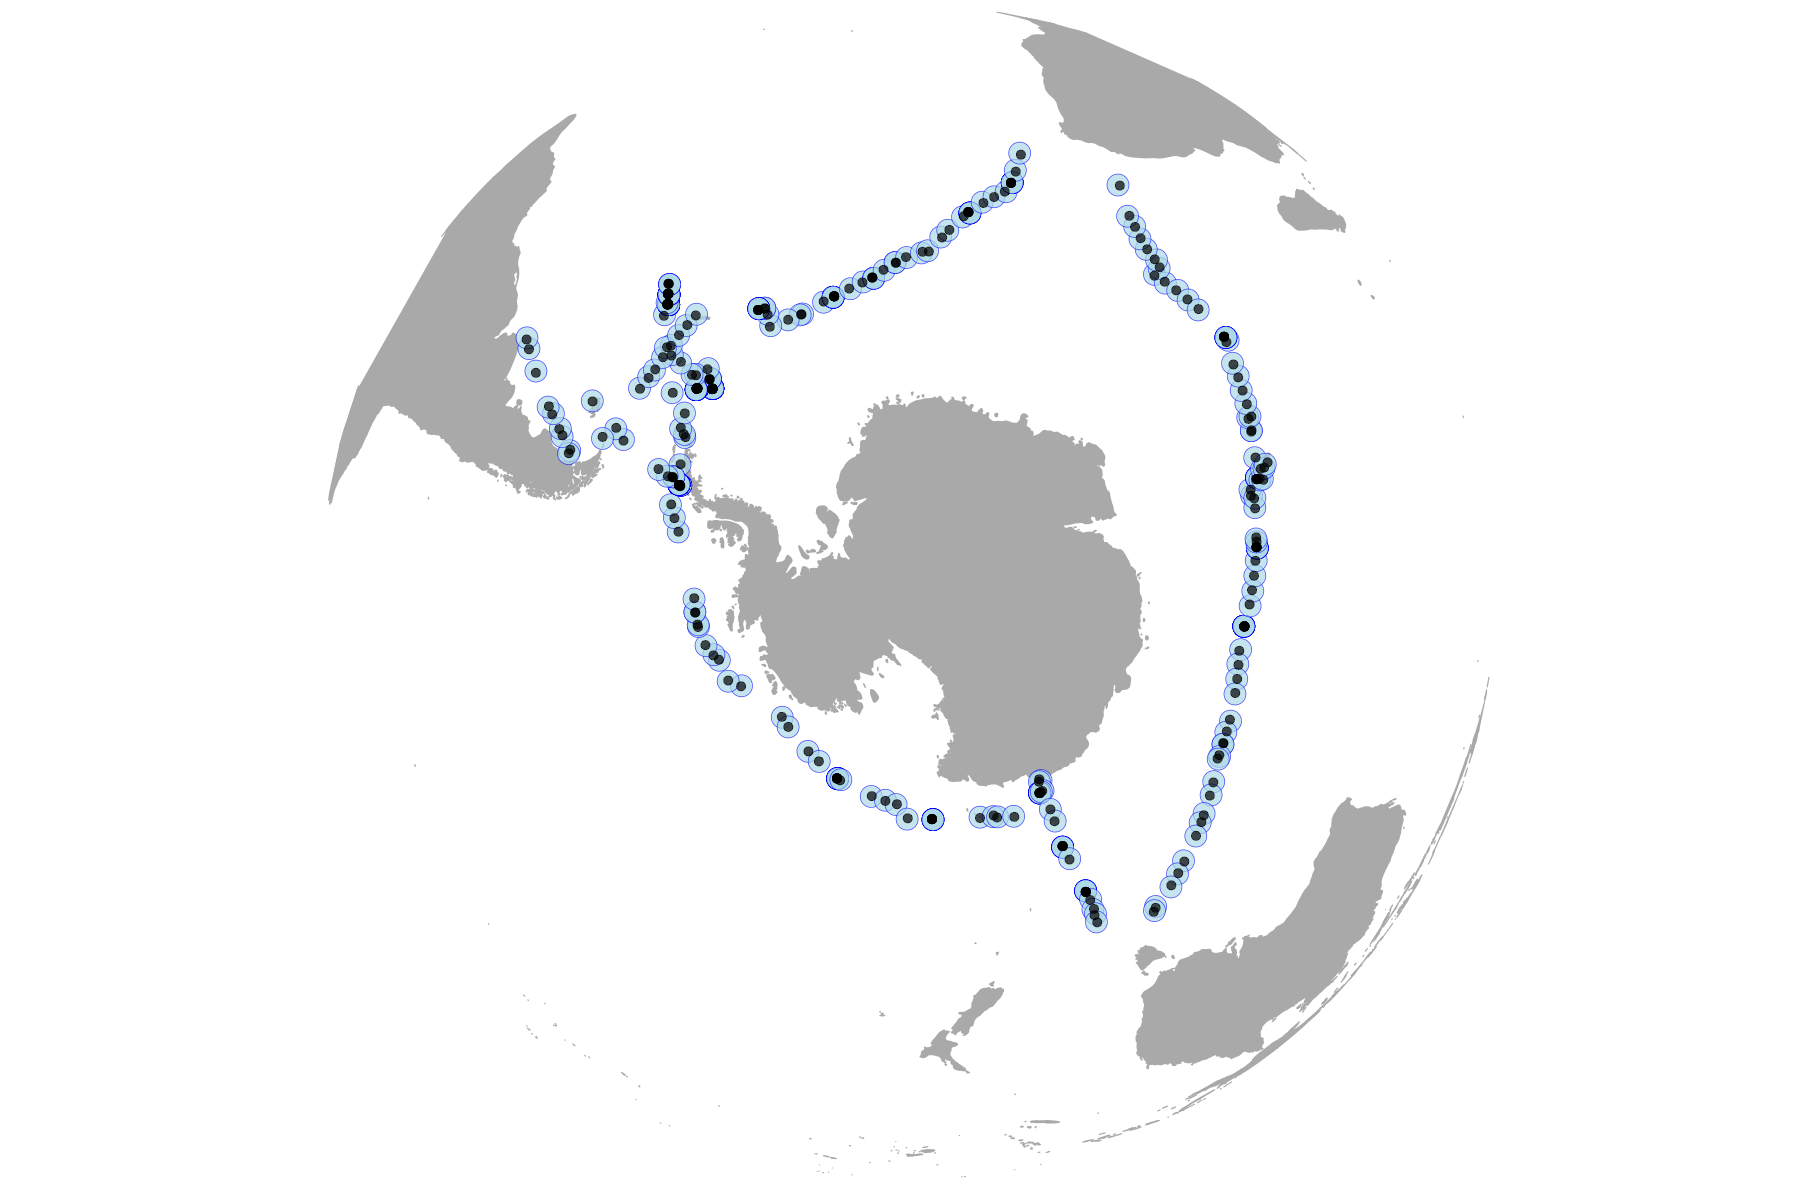
\includegraphics[width=.8\textwidth]{Plots/validation_isoprene_roms_bec_ant.png}
\caption{Sampling points used for validation. Data were recompiled from three different research cruises: TransPEGASO, PEGASO and ACE Expedition. }
\label{fig:cruises}
\end{figure}

\subsubsection{GC-MS Data}
\textbf{\textit{GC-MS Protocol}}
Data of isoprene concentration in the sea surface of the antarctic ocean were obtained using a Agilent TM GC-MS (gas chromatography mass spectrometry) during the mentioned oceanographic cruises. For both cruises, the surface data were sampled from underwerway systems, CTDs and Day-night cycles of 36 hours. \\

\subsubsection{Pigments and Chlorophyll}

Pigment data from HPLC-CHEMTAX were used to validate the model results.\\
Chla from ACE --> David Antoine Group.\\
Chla from PEGASO --> Marta Estrada Group.\\
Total Chl-a was discretely sampled and processed according to XXXXX during PEGASO and ACE Projects. Also, HPLC data were obtained.\\
PEGASO cruise: Sdena Nunes and Marta Estrada Group (ask for description).\\
ACE cruise: Needed from Antoine's group (ask for description).\\

\subsection{Production rates of isoprene from PEGASO \textit{in situ} data}

We calculated isoprene production rates for the PFT included in the model based on in situ data. During PEGASO cruise (2015) we performed four bloom site lagrangian studies (36 hours each) in different locations of the SO (Orkney Islands, Weddel Sea, South Georgia Islands and Gerlache Strait).
These location were selected because they were under bloom conditions.
In previous works \citep{meskhidze2006phytoplankton} other authors have measured high emission of VOCs in these areas.
Every 30' we intensively sample isoprene concentration. Also, we sampled every 4 hours for isoprene concentration, and other environmental and biological associated variables, in order to characterize phytoplankton communities.
Therefore, we could see the variation of isoprene concentration along 36 hours under different areas in the SO in bloom conditions.
Despite this was a not a culture experiment, as reported in many other works \citep{shaw2003isoprene,exton2013chlorophyll,booge2016can}, here we propose and alternative calculus to obtain isoprene PFT production rates.

First we calculated the flux of isoprene according to \citep{palmer2005quantifying}:\\

\begin{linenomath*}
\begin{equation}
F_{Iso} = k_{AS} \cdot (Iso_{w} - \frac{Iso_{w}}{K_{H}}) = ∼ k_{AS} \cdot Iso_{w}
\end{equation}
\end{linenomath*}

We used $K_{AS}$ approach firstly described in \citep{palmer2005quantifying} and the Schmidtt number from \citep{wanninkhof1992relationship}.\\

\begin{linenomath*}
\begin{equation}
k_{AS} = 0.31 \cdot U_{10}^{2} \bigg(\frac{Sc}{660}\bigg)^{-0.5}
\end{equation}
\end{linenomath*}

\begin{linenomath*}
\begin{equation}
Sc = 3913.15 - (162.13 \cdot T) + (2.67 \cdot T^{2}) - (0.012 \cdot T^{3})
\end{equation}
\end{linenomath*}

Where \textit{T} ins temperature in Degrees Celsius.\\

Therefore, the daily (per day) isoprene budget is defined as follows according to \citep{booge2016can}. A broader description of the parameters can be seen in Table \ref{tab:pegrates}.\\

\begin{linenomath*}
\begin{equation}
\frac{ΔIso_{w}}{d} =  P - \overline{Iso}_{w} \cdot (Σ k_{CHEM, i} C_{xi}) - \overline{Iso}_{w}  \cdot k_{BIOL} - \frac{F_{Iso}}{MLD} - L_{MIX}
\end{equation}
\end{linenomath*}

Where $P_{Iso}$ is isoprene production, $\overline{Iso}_{w}$ is the mean of isoprene concentration in sea water all over the experiment, $k_{chem, i}$ chemical rate constant for all possible loss pathways (i) with all reactants (X) (X = OH and O 2 ), $k_{BIOL}$ is the biological degradation rate of isoprene by bacteria, $F_{Iso}$ is the isoprene flux to the atmosphere, \textit{MLD} is the mixing layer depth and $L_{mix}$ is the loss due to mixing constant. 
Note that all rates are positive. In case  $L_{mix}$represents an income into the \textit{MLD} from a concentration maximum below, take $L_{mix}$ as negative.

Therefore, for every bloom diel-cycle of 36 hours:\\

\begin{linenomath*}
\begin{equation}
P_{Iso} = \frac{ΔIso_{w}}{d} + \overline{Iso}_{w} \cdot (Σ k_{CHEM, i} C_{xi}) + \overline{Iso}_{w} \cdot k_{BIOL} + \frac{F_{Iso}}{MLD} + L_{MIX}
\end{equation}
\end{linenomath*}

Now, having the isoprene production \textit{P} we are able to calculate the daily production rate of isoprene per chlorophyl.\\

\begin{linenomath*}
\begin{equation}
P_{ISO.CHLA} = \frac{P_{ISO}}{CHLA}
\end{equation}
\end{linenomath*}

\begin{center}
\begin{table}[h!]
\centering
\caption{Parameters of the PFT isoprene production rates calculated from \textit{in situ} data in four different blooms in the SO.}
\label{tab:pegrates}
\begin{tabular}[ht]{ c|c|c|c|c|c } 

 \textbf{Parameter} & \textbf{Unit} & \textbf{Description} & \textbf{Value} & \textbf{Variability} \\\hline
 $\mathrm{P_{ISO.CHLA}}$   &  $\mathrm{pmol} \; \mathrm{L}^{\mathrm{-1}} \; \mathrm{d}^{\mathrm{-1}}\; \mathrm{mg chla}^{\mathrm{-1}}$  & \tiny{isoprene production per chlorophyll} &  -  & -  \\

 $\mathrm{P_{ISO}}$   &  $\mathrm{pmol} \; \mathrm{L}^{\mathrm{-1}} \; \mathrm{d}^{\mathrm{-1}}$  & \tiny{isoprene production} &  -  & - \\

$\mathrm{F_{ISO}}$     & $\mathrm{pmol} \; \mathrm{m}^{\mathrm{2}} \; \mathrm{d}^{\mathrm{-1}}$   & \tiny{isoprene flux} & - & -  \\

$\mathrm{K}_{\mathrm{BIO}}$ & $\mathrm{d}^{\mathrm{-1}}$ & \tiny{Biological loss rate} & 0.06 & 0 - 0.06 \\

$\mathrm{k}_{\mathrm{CHEM, x}} \cdot \mathrm{C}_{\mathrm{x, i}}$ & $\mathrm{d}^{\mathrm{-1}}$ & \tiny{Chemical loss rates of O2 and OH } & 0.0518 & -  \\

$\mathrm{MLD}$ & m & \tiny{Mixing Layer Depth} & - & - \\

$\mathrm{\frac{ΔIso_{w}}{d}}$ &  $\mathrm{pmol} \; \mathrm{L}^{\mathrm{-1}} \; \mathrm{d}^{\mathrm{-1}}$ & \tiny{Change in Isoprene concentration over 24 hours} & - & - \\

$\mathrm{\overline{Iso}_{w}}$ &  $\mathrm{pmol} \; \mathrm{L}^{\mathrm{-1}}$ & \tiny{Mean of isoprene concentration on every bloom} & - & - \\

\end{tabular}
\end{table}
\end{center}

\begin{center}
\begin{table}[b!]
\caption{Isoprene production PFT rates on every bloom.}
\centering
\label{tab:pegblooms}
\begin{tabular}[ht]{ c|c|c|c|c|c } 

 \textbf{Bloom} & \textbf{Area} & \textbf{ $\mathrm{P_{CHLA}}$ }& \textbf{Units} & \textbf{Dominant PFT} \\\hline
 I &  Orkney Islands & 3.32   &  $\mathrm{pmol} \; \mathrm{L}^{\mathrm{-1}} \; \mathrm{d}^{\mathrm{-1}}\; \mathrm{mg chla}^{\mathrm{-1}}$& 26\% haptophytes, 37\% cryptophytes  \\
II &   Weddell Sea&  11.06   &  $\mathrm{pmol} \; \mathrm{L}^{\mathrm{-1}} \; \mathrm{d}^{\mathrm{-1}}\; \mathrm{mg chla}^{\mathrm{-1}}$ &  80\% haptophytes\\
 III &  South Georgia Islands & 4.11   &  $\mathrm{pmol} \; \mathrm{L}^{\mathrm{-1}} \; \mathrm{d}^{\mathrm{-1}}\; \mathrm{mg chla}^{\mathrm{-1}}$  & 80\% diatoms  \\
 IV & Gerlache Strait & 1.78   &  $\mathrm{pmol} \; \mathrm{L}^{\mathrm{-1}} \; \mathrm{d}^{\mathrm{-1}}\; \mathrm{mg chla}^{\mathrm{-1}}$  &  57\% cryptophytes, 24\% haptophytes\\

\end{tabular}
\end{table}
\end{center}

In base to HPLC data, we determined that each of the blooms was dominated by different phytoplankton species Table \ref{tab:pegblooms}.

\subsection{Model description}

Extract model forcing from \citep{Nissen2018}.\\

The phytoplankton community structure in the southern ocean  is dominated by coccolitophores and diatoms.

In one hand, \textbf{Coccos}: Coccolitophores species dominate the phytoplankton communities among 40-60 S, covering an area which is known as the "Great Calcite Belt" \citep{balch2011contribution}. In the model, we selected PFT rates of different strains of \textit{Emiliana huxleyi}, compiled in \citep{booge2016can}, since is is the dominant species among southern ocean coccolitophores \citep{Saavedra-Pellitero2014, balch2016factors}.

In the other hand, \textbf{Diatoms}: Diatoms are the dominant species of phytoplankton southern than 60 S \textbf{RERF}.

\textbf{Small phytoplankton}: We selected the baterioplankton spcies, Prochlorococcus sp. \& Synechococcus sp. , as the main contributors to the "Small Phytoplankton" budget. Despite they are not the most abundant species in the high latitudes of the southern ocean, they dominate many areas among 30 and 40 degrees \textbf{REF}.

\begin{center}

\begin{table}[h!]

\centering

\caption{Parameters related to isoprene tracer in BEC. The isoprene production rate of diatoms and coccolithophores includes measurements of cold adapted diatoms and \textit{Emiliania huxleyi} only, respectively. \textbf{REF} Variability is only given when multiple values are reported in the cited literature.  \textbf{check units!!}}

\label{tab:params}

\begin{tabular}[ht]{ c|c|c|c|c|c } 

 \textbf{Parameter} & \textbf{Unit} & \textbf{Description} & \textbf{Value} & \textbf{Variability} & \textbf{Ref} \\\hline

 $\rho^{\mathrm{Diat}}_{\mathrm{chl}}$     & $\mathrm{mmol} \; \mathrm{mgChl}^{\mathrm{-1}} \; \mathrm{d}^{\mathrm{-1}}$  & \tiny{isoprene production rate of diatoms (cold adapted ones)} & 2.06 & 0.56-9.36 &  \citet{booge2016can} \\

$\rho^{\mathrm{Cocco}}_{\mathrm{chl}}$     & $\mathrm{mmol} \; \mathrm{mgChl}^{\mathrm{-1}} \; \mathrm{d}^{\mathrm{-1}}$   & \tiny{isoprene production rate of coccolithophores (E. huxleyi)} & 5.54 & 1-11.28 & \citet{booge2016can}  \\

$\rho^{\mathrm{SP}}_{\mathrm{chl}}$     & $\mathrm{mmol} \; \mathrm{mgChl}^{\mathrm{-1}} \; \mathrm{d}^{\mathrm{-1}}$  & \tiny{isoprene production rate of small phytoplankton (Prochloroccus + synecho} & 5.73 & 1.4 &  \citet{booge2016can} \\

$\mathrm{Loss}_{\mathrm{Bio}}$ & $\mathrm{d}^{\mathrm{-1}}$ & \tiny{Biological loss rate} & 0.06 & 0 - 0.06 &  \citet{booge2016can}\\

$\mathrm{k}_{\mathrm{OH}} \cdot \mathrm{C}_{\mathrm{OH}}$ & $\mathrm{d}^{\mathrm{-1}}$ & \tiny{Chemical loss rate (OH) } & 0.0518 & - & \citet{booge2016can} \\

$\mathrm{k}_{\mathrm{O_{\mathrm{2}}}} \cdot \mathrm{C}_{\mathrm{O_{\mathrm{2}}}}$ & $\mathrm{d}^{\mathrm{-1}}$ & \tiny{Chemical loss rate (O2)} & 0.0009 & - & \citet{booge2016can} \\

\end{tabular}

\end{table}

\end{center}

We run our simulations in the SO setup of ROMS-BEC \citep{Haumann2016,Nissen2018} which is a mechanistic marine ecosystem model in terms of phytoplankton dynamics in the Southern Ocean (circumpolar, ranging from the Antarctic continent to 24deg S) in the 0.5 degree setup (appr. 10-50km horizontal resolution) and 64 sigma layers in the vertical.
\textbf{Give a general description of BEC along these lines: } BEC is modeling the biogeochemical cycles of C, N, P, Si and O$_{2}$. It has three phytoplankton (diatoms, coccolithophores and a mixed small phytoplankton group) and one zooplankton PFT. A more detailed description is given in \citet{Moore2013} and \citet{Nissen2018} for the version specifically tuned for the SO setup that is used here. 

For this study, we implemented isoprene as an additional tracer. We calculated the isoprene concentration, production and emission by following \citet{palmer2005quantifying, booge2016can}. 
Changes of isoprene concentrations over time are dependent on production and loss terms (see Eq. \ref{eq:disodt}).
Isoprene in ROMS-BEC is produced by the phytoplankton PFTs ($\mathrm{P}_{\mathrm{PFT}}$) and loss processes include a biological loss ($\mathrm{L}_{\mathrm{bio}}$, accounting for bacterial consumption), chemical loss ($\mathrm{L}_{\mathrm{chem}}$, reaction with radicals) and loss to the atmosphere ($\mathrm{L}_{\mathrm{atm}}$):

\begin{linenomath*}
\begin{equation}
\frac{\mathrm{d \, ISO}}{\mathrm{dt}} = \mathrm{P}_{\mathrm{PFT}} - \mathrm{L}_{\mathrm{BIO}} - \mathrm{L}_{\mathrm{CHEM}} - \mathrm{L}_{\mathrm{ATM}}
\label{eq:disodt}
\end{equation}
\end{linenomath*}

Isoprene production is linearly coupled to phytoplankton chlorophyll levels, with the constant rate being specific to each PFT (Table \ref{tab:params}):
\begin{linenomath*}
\begin{equation}
\mathrm{P}_{\mathrm{PFT}} = \sum^{3}_{i=1}\rho^{i}_{chl} \cdot [PFT^{i}_{CHLA}]
\label{eq:ppft}
\end{equation}
\end{linenomath*}
Here, the diatom value is the average of the cold adapted diatoms in \citet{booge2016can} only, and the coccolithophore value is the average over all \textit{Emiliana huxleyi} values in \textbf{REF}, accounting for the fact the this species dominates the SO phytoplankton community \citep{Smith2017,Saavedra-Pellitero2014}. For SP and diazotrophs, we take a small production ratio because \textbf{bla bla}.

\begin{linenomath*}
\begin{equation}
\mathrm{L}_{\mathrm{BIO}} = [Iso]_{w} \cdot K_{BIO}
\label{eq:latm}
\end{equation}
\end{linenomath*}

The loss rates are constant and taken from \textbf{REF}, the only study reporting these values:
\begin{linenomath*}
\begin{equation}
\mathrm{L}_{\mathrm{CHEM}} = [ISO]_{w} \cdot K_{CHEM}
\label{eq:lchem}
\end{equation}
\end{linenomath*}

The ocean is supersaturated with respect to the atmosphere, and the ocean-atmosphere flux can be written as: 
\begin{linenomath*}
\begin{equation}
\mathrm{L}_{\mathrm{ATM}} = [ISO]_{w} \cdot K_{AS}
\label{eq:lbio}
\end{equation}
\end{linenomath*}

\textit{KAs} is the gas exchange coefficient according to \citet{wanninkhof1992relationship}:
\begin{linenomath*}
\begin{equation}
k_{AS} = 0.31U^{2} \left(\frac{S_{C}}{660}^{-0.5}\right)
\label{eq:kas}
\end{equation}
\end{linenomath*}

\textbf{Notes (Cara):}
Here, all the formula need to be explained a bit better and assumptions need to be stated. Where do phytoplankton produce isoprene? Is it excreted instantaneously or does some remain "attached"/incorporated in the cell? If so, what happens if phytoplankton dies? Meike noted that it might be worth to test a different formulation for the gas exchange - just to get a feeling for how much that impacts our emission estimate. She also noted that it needs to be stated more clearly what the different constants (especially the loss terms) represent.

We selected the cold adapted diatoms instead (lower production rates values from ~3 to ~2, cocolitophores and diazotrophs.\\
Advection (Lmix) and MLD, were solved from ROMS-BEC physical compartment.\\

\subsection{Sensitivity tests}
\begin{table}
\caption{Overview of simulations for this study. See Table \ref{tab:params} for values in baseline simulation.}
\label{tab:model_runs}
\centering
%\resizebox{\textwidth}{!}{%
\begin{tabular}{ l l l l l} 
\hline
 & \textbf{Run Name} 		& \textbf{Description} 	   & \textbf{Value}  & \textbf{Units}\\\hline
1 & Baseline			   	& Same as in \citet{Nissen2018}, isoprene parameters like in Table \ref{tab:params}  & XXXXX &Tg C yr -1\\
2 & high\_bio\_loss 		&  k$_{\mathrm{loss}}^{\mathrm{bio}}$ = 0.06 &  XXXXX &Tg C yr -1 \\
3 & low\_bio\_loss 		&  k$_{\mathrm{loss}}^{\mathrm{bio}}$ = 0.01 & XXXXX &Tg C yr -1\\
4 & high\_PFT\_prod 		& Set all PFT iso prod. rates to upper range given in Table \ref{tab:params}   & XXXXX  &Tg C yr -1\\
5 & low\_PFT\_prod 		    &  Set all PFT iso prod. rates to lower range given in Table \ref{tab:params} & XXXXX &Tg C yr -1\\
4 & Pegaso PFT +  k$_{\mathrm{loss}}^{\mathrm{bio}}$ = 0.06		& PFT production rates obtained from PEGASO Cruise \ref{tab:params}   & XXXXX  &Tg C yr -1\\
5 & Pegaso PFT +  k$_{\mathrm{loss}}^{\mathrm{bio}}$ = 0.01       & PFT production rates obtained from PEGASO Cruise\ref{tab:params} &  XXXXX &Tg C yr -1\\
6 & Pegaso PFT +  k$_{\mathrm{loss}}^{\mathrm{bio}}$ = 0.06       & Diatoms Southern Ocean (\citep{booge2016can})\ref{tab:params} & XXXXX  &Tg C yr -1\\
... & ... & ... & ... & \\
X & high\_chem\_loss 		&  Increase k$_{\mathrm{loss}}^{\mathrm{chem}}$ by \textbf{XX}\% & XXXXXX &Tg C yr -1\\
X & low\_chem\_loss 		&  Decrease k$_{\mathrm{loss}}^{\mathrm{chem}}$ by \textbf{XX}\% & XXXXX &Tg C yr -1\\
\hline
\end{tabular}%}
\end{table}

We supply surface initial conditions of isoprene concentration as monthly climatologies applying the equation proposed by \citep{hackenberg2017potential} to MODIS sea surface temperature and chlorophyll-a monthly climatologies. Below the surface (for both initial fields and the boundary conditions), we assume a constant value of XX. Given isoprene's typical range of XX-XX in the SO (reference to your data?), this value is rather a low value. \\

We first do a physics only spin up of 30 years. The baseline run is 20 years long and we analyze the monthly climatology of year 15-20. Each of the sensitivity simulations is started from the 10-year restart file of the baseline run, and then run for ten years. As for the baseline, we assess the monthly climatology of year 5-10.

In the sensitivity runs, we assess the sensitivity to chosen parameters as shown in \ref{tab:params}. We increase and decrease the PFT production rates according to the variability reported in the literature and vary the values by \textbf{XX}\% for the others. \textbf{Elaborate on this.} 

- Model validation: Sensitivity tests. What is interesting to test? Mostly Kbiol and Kchem, that means the constants of biological and chemical degradation respectively. Why? Because they are the variables of which we have a lack of knowledge. Also, in order to perform future experiments (in our group or other) this can point out what are the main uncertainties to solve.\\

\textbf{Cara and Meike suggest} to perform sensitivity tests on all the model parameters, which is what they usually do:\textit{ For instance, the PFT production rates are also prone to substantial uncertainties, and need to be assessed in terms of model sensitivity, especially since the integrated emissions are our target variables, and these will depend both on sources and sinks.}

- How we do that? We need the monthly climatology of the model (of how many years, lets say 10?). After we compare our in situ data (with latitude and longitude information) with the model data. The key variable to compare is isoprene concentration, since it is the variable we have in situ measured. Regarding to the temporal resolution of the model: ideally in the same moment of the sampling (hourly or daily), however we have already seen in the model output that a weekly basis is fine (actually in the most productive months, when blooms arrive(dec-feb), the intra monthly variation is higher, being possible to observe the south georgia bloom).\\

\textbf{Cara and Meike suggest}: \textit{Usually, we start from literature uncertainty estimates, and if these don't exist, we use educated guesses by experts, i.e. ask Rafel which uncertainty ranges he deems likely. If we can't put a number on this, we vary all constants by a fixed amount, e.g. +- 50\%, +- 10\% etc. to assess model sensitivity. In terms of th e model output, we will need to test different temporal aggregation scales. For instance, model output can be produced at the daily scale and matched with observations, but if the uncertainties are high, and the variables to be assessed highly variable and heterogeneous in space, a higher degree of spatio-temporal averaging might be advantageous. The model cannot reproduce detailed patterns of highly fluctuating variables, so comparing in a point-to-point fashion would be a little unfair to the model. We can discuss this while you're here once we see how the model-data misfit looks like.}\\

\section{Results}

The main purpose/ultimate goal of this work, should be to quantify the {relative contribution of the Southern Ocean to the global emissiones of marine isoprene}. 

\subsection{Isoprene patterns in space (model evaluation)}
In this section, we describe the spatial patterns produced by ROMS-BEC.

\begin{itemize}
\item Spatial patterns of surface annual mean isoprene concentrations (Observations plotted on top!). Consider plotting the top \textbf{XX}m mean instead of surface only (Fig. \ref{fig:spatial}A). 
\item Zonal avg depth distribution (example profile from observations?) (Fig. \ref{fig:spatial}B). 
\item Map of annually integrated marine isoprene emissions (Fig. \ref{fig:emissions_map}).
\end{itemize}

\textbf{Notes (Cara):}
Here, I would focus on the large scale patterns. Don't get hung up on small scale structures. The model has a positive chlorophyll bias at high SO latitudes, resulting partly from too high temperatures and too shallow MLD (ask me to send the latest version of my first paper, a more detailed description/discussion about biases is in there), so this will affect the isoprene estimates as well. Production of isoprene at high SO latitudes is expected to be too high because of too high diatom production at these latitudes. How much this bias at high latitudes will contribute to integrated isoprene estimates will depend on how important this area is for total isoprene production (to be computed).
For the distribution of isoprene with depth, I am curious to see a typical profile that you have measured. Here, it will matter that modeled ML tend to be too shallow, so phytoplankton production (and hence isoprene production) likely doesn't occur as deep as in observations.
For the emissions, keep in mind that these are a function of wind speed etc. and are scaled by any ice cover in each grid cell. For example, the blue patch in the Weddell Sea of almost zero emissions is very likely an area where sea ice cover is high all year round in our model. So as you can see, this area of almost zero emissions is an area of high isoprene concentrations (it simply accumulates there and cannot escape).

\begin{figure}[h]
\centering
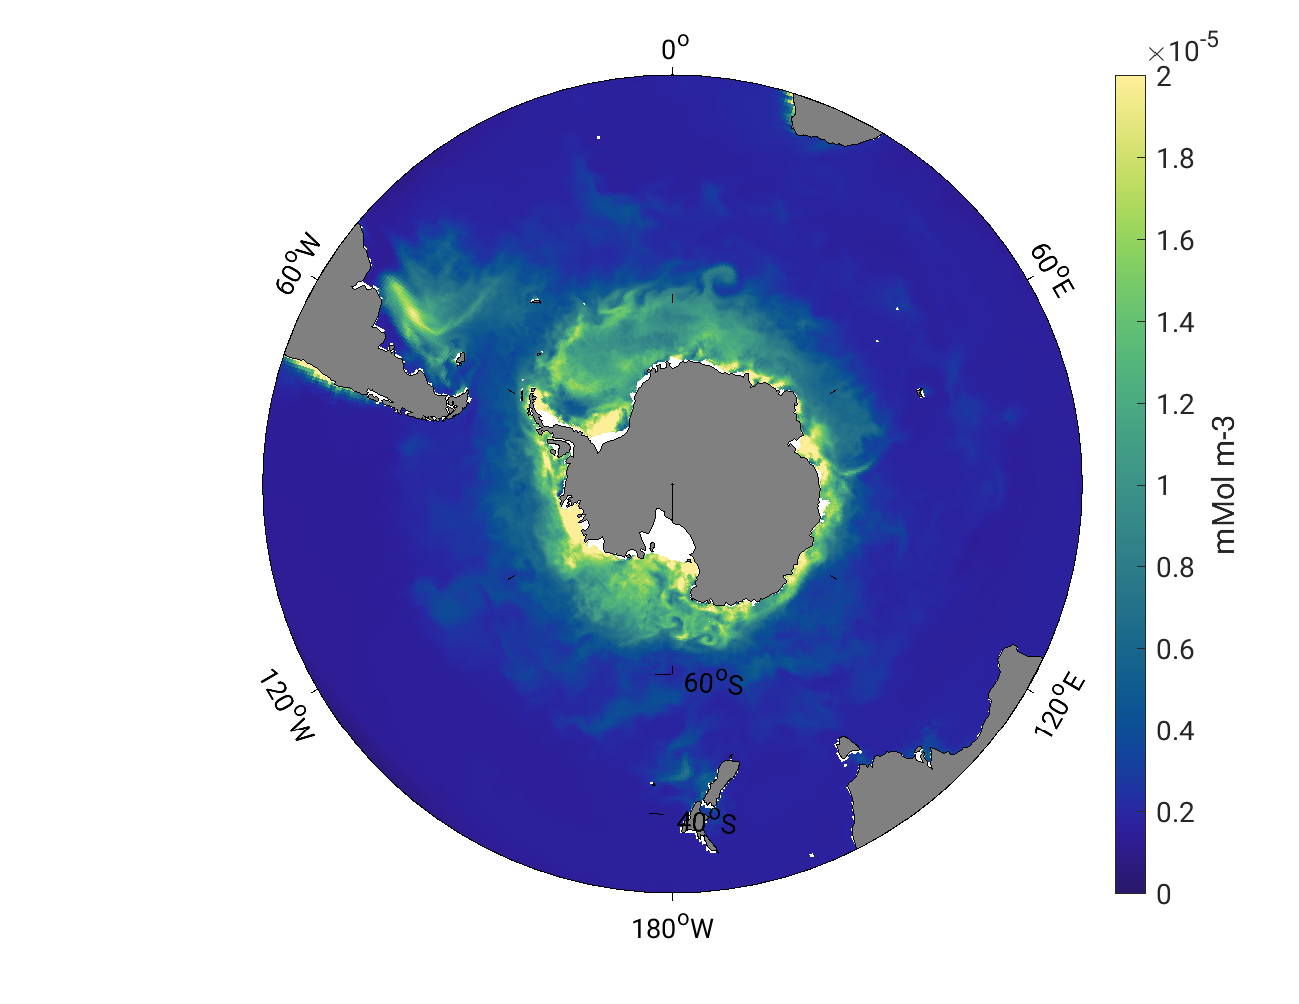
\includegraphics[width=.4\textwidth]{Plots/ISOPRENE_annual_at_10m_031.png}
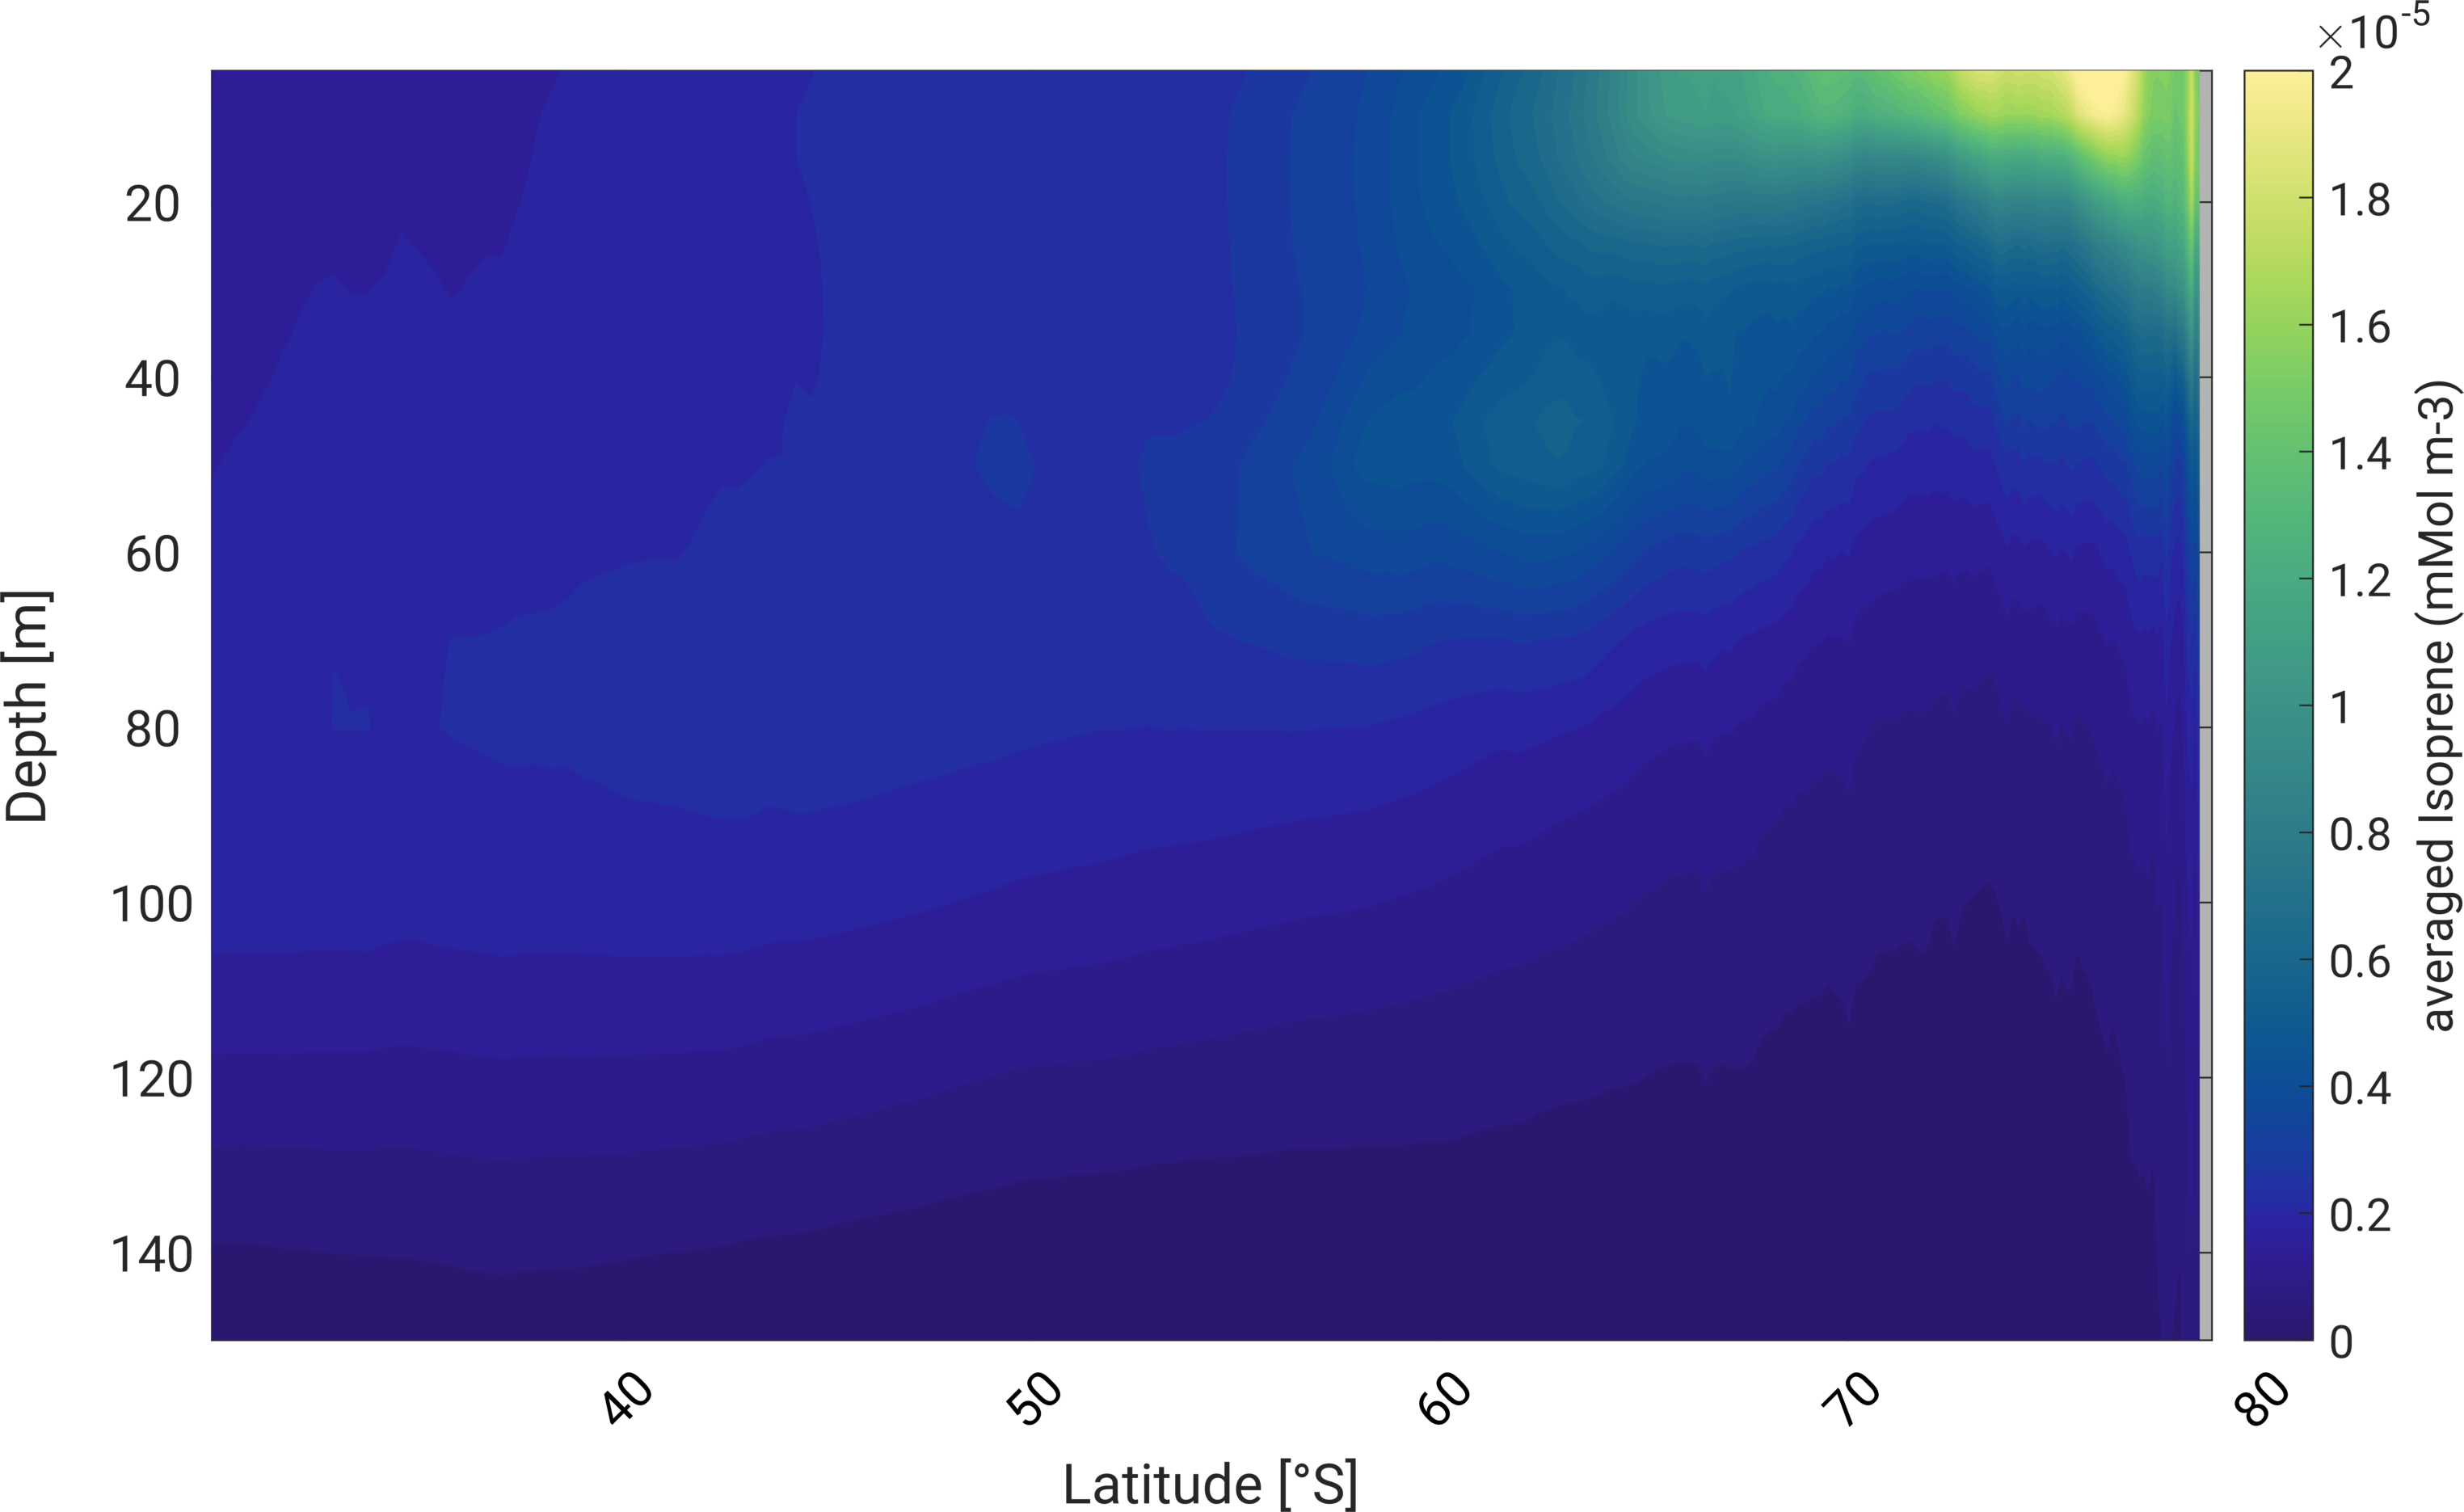
\includegraphics[width=.4\textwidth]{Plots/Zonal_avg_annual_mean_ISOPRENE_031_clm.png}
\caption{Annual mean surface isoprene concentrations \textbf{(left)} and annual mean zonally averaged depth distribution of isoprene concentrations \textbf{(right)}. Note the log scale}
\label{fig:spatial}
\end{figure}

\begin{figure}[h]
\centering
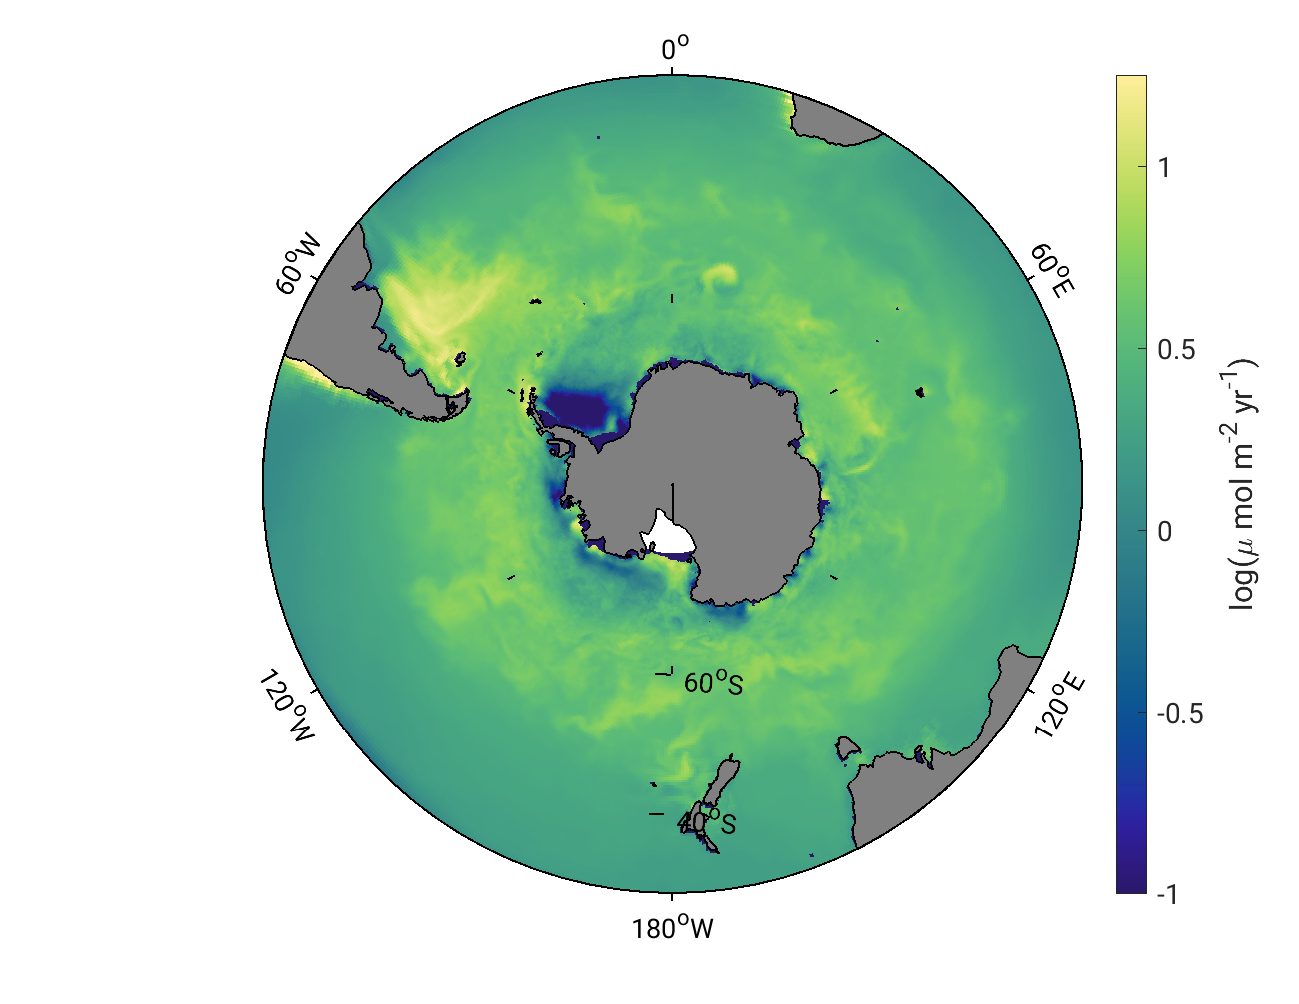
\includegraphics[width=.6\textwidth]{Plots/Isoprene_emissions_annual_031.png}
\caption{Spatial distribution of annually integrated isoprene emissions. Note the log scale.}
\label{fig:emissions_map}
\end{figure}



\subsection{Isoprene patterns in time}
In this section, we describe the temporal dynamics of isoprene produced by ROMS-BEC.
\begin{itemize}
\item temporal/seasonal dynamics of fluxes (Fig. \ref{fig:emissions_ts})
\item Hovm{\o}ller plots: Phyto iso production vs iso emissions (zonal avg: lat vs month, is there differences between basins?) (Fig. \ref{fig:hovmoller})
\end{itemize}

\textbf{Notes (Cara):}
I would suggest to also plot the seasonality of chlorophyll (I expect pretty much the same seasonality), just to get a feeling for what the model does. Generally, peak chlorophyll is too early at high latitudes (it's too warm and too bright - so phytoplankto love it there! see my first paper), so again, isoprene peak production is also expected too early there. How that effects the domain integrated seasonality as shown in the figure...?? I have to think about this. But it will depend on how dominant the high latitudes are.
As discussed with Meike, here we are e.g. also interested in whether there is a temporal lag in maximum isoprene production and maximum emissions (see Hovmoller plot). We will get nicer plots once the daily output is ready... For these plots, consider also that isoprene is transported around by physics, so where isoprene is produced is not necessarily where all of it escapes to the atmosphere.

\begin{figure}[h]
\centering
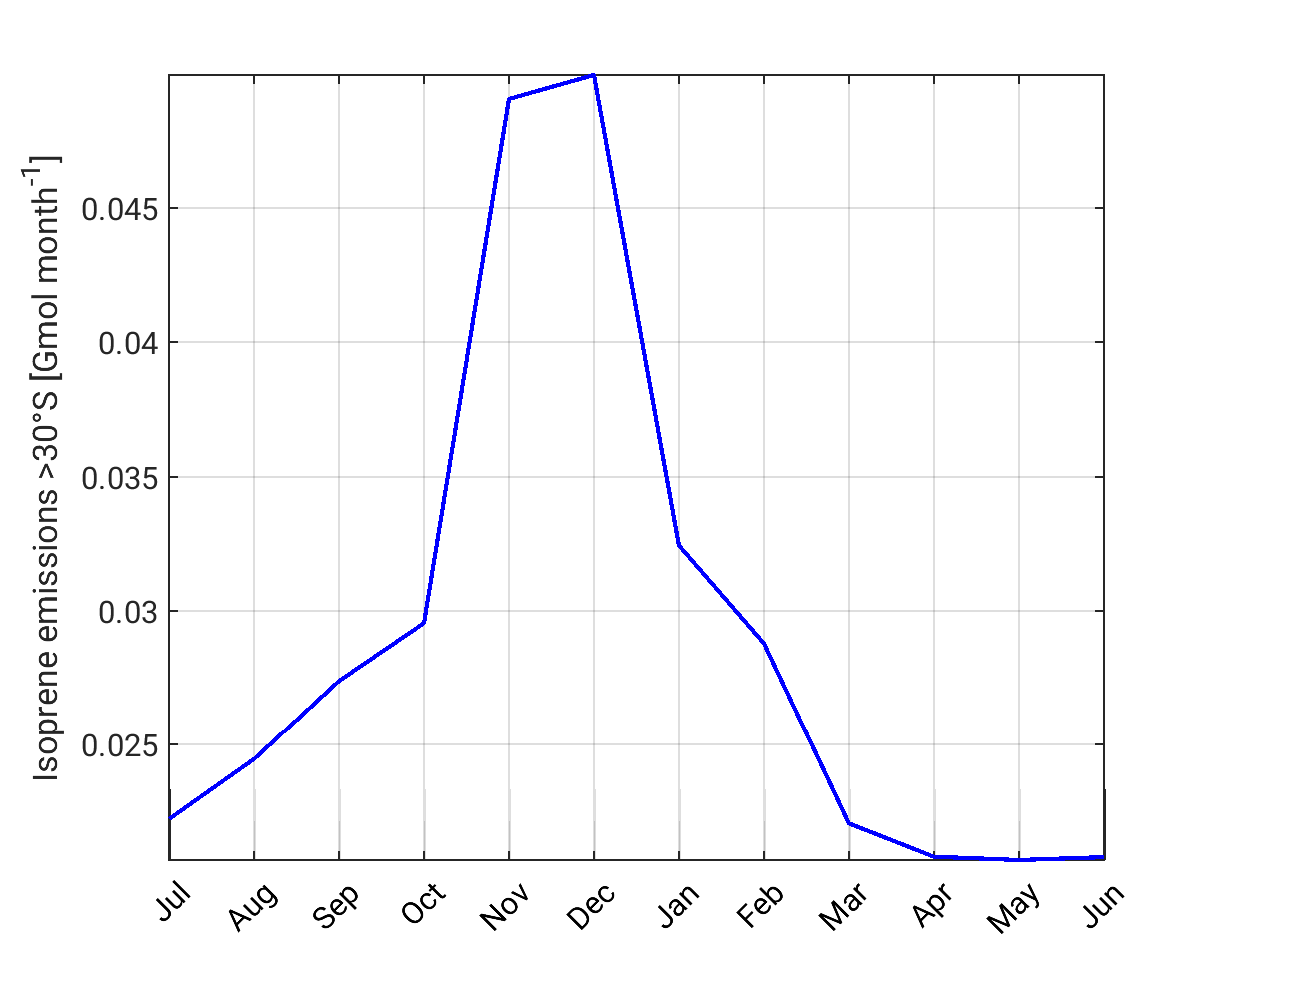
\includegraphics[width=.6\textwidth]{Plots/Isoprene_emissions_monthly_timeSeries_031.png}
\caption{Time series of monthly integrated isoprene emissions for the area south of 30$^{\circ}$S. \textbf{Idea: add shading around the curve corresponding to range of emissions for each month as obtained by the suite of parameter sensitivity simulations!}}
\label{fig:emissions_ts}
\end{figure}

\begin{figure}[h]
\centering
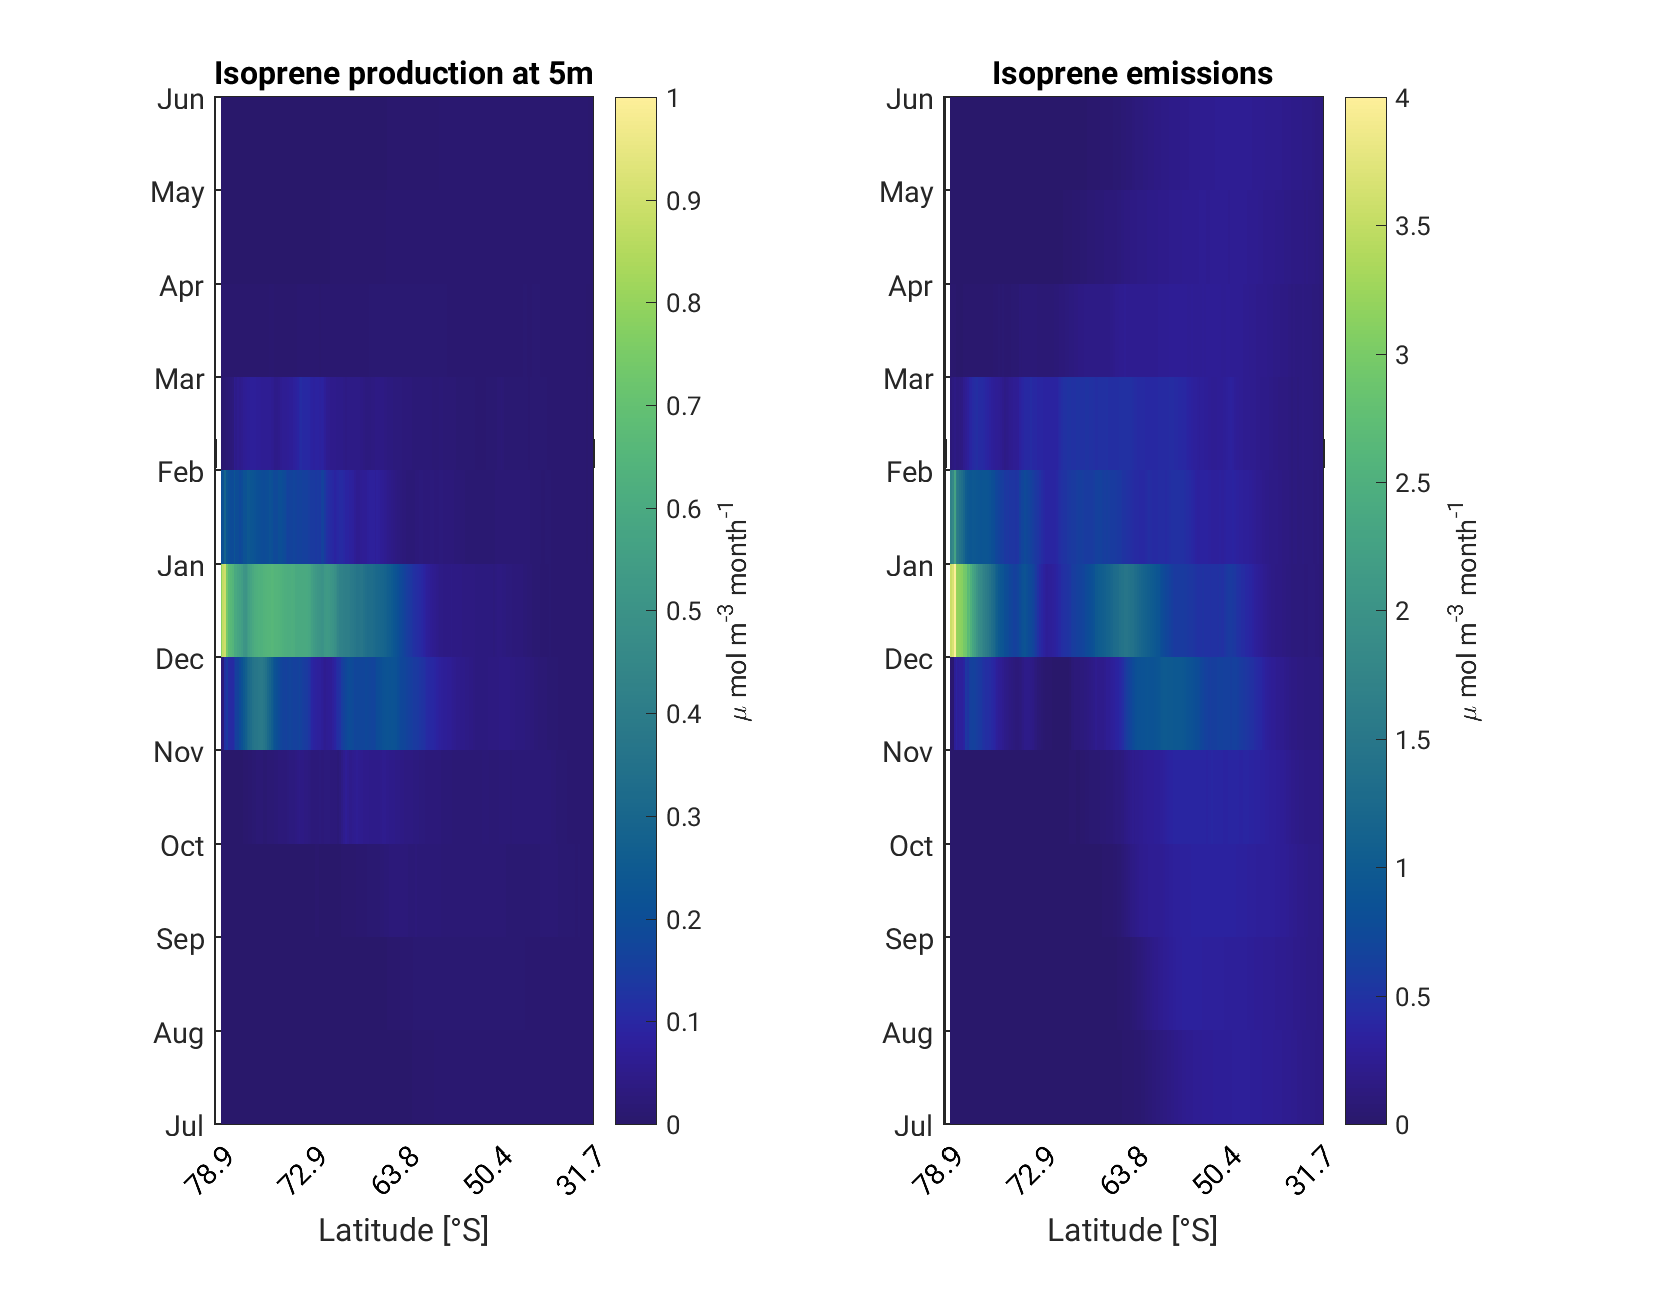
\includegraphics[width=.9\textwidth]{Plots/Hovmoller_031_isoprene_prod_at_5m_srf_flux_circumpolar.png}
\caption{Hovm{\o}ller diagram of zonally averaged total isoprene production at 5m \textbf{(left)} and surface isoprene emissions \textbf{(right)} as a function of time. \textbf{This plot will look a lot better with daily output! Think about whether to plot production at one depth level or depth integrated production.}}
\label{fig:hovmoller}
\end{figure}


\subsection{Biogeochemical implications: Integrated marine isoprene emissions}
\begin{itemize}
\item Table with integrated emission estimates
\item Set integrated emission estimates for SO domain into context with previously published global estimates. 
\end{itemize}
\textbf{Notes (Cara):}
Here, it will be interesting to see the estimates for different latitudinal bands, first of all, to get an idea of how important the different regions are, but second of all, to then also relate that to possible biases in the different regions (see my first paper).
Additionally, here I think it could be interesting to apply the satellite derived algorithms on the model output (SST, total chl,...?) and compare it to the emission estimate calculated dynamically in ROMS. 

\subsection{Sensitivity simulations}
\begin{itemize}
\item How does uncertainty in parameters impact results?
\item Which are the parameters the model output (meaning integrated emission estimates, as well as e.g. mean concentrations/inventory?) is most sensitive to?
\end{itemize}
\textbf{Notes (Cara):}
Calculate the integrated emissions for each of the runs and have a look for which run it changes most in the different areas. Is it the same parameters in all areas or do you find differences? 

\subsection{Validation}


\begin{figure}[h]
\centering
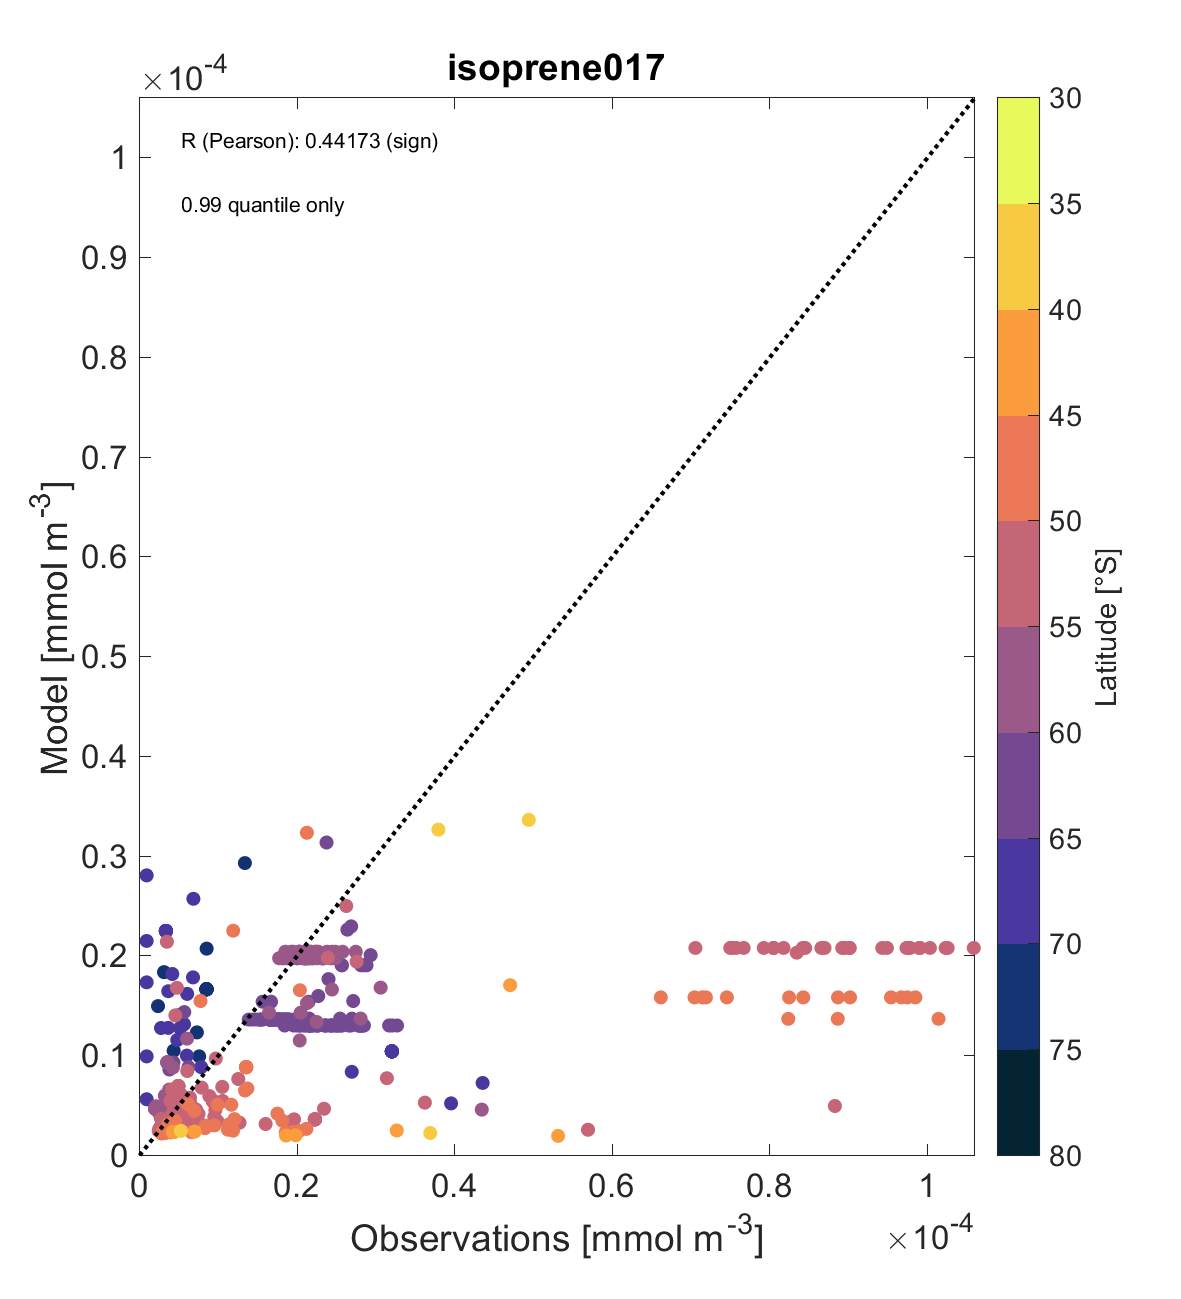
\includegraphics[width=.9\textwidth]{Plots/isoprene_observations_vs_modelo_017_3080_2_Lat_099_PAPER.png}
\caption{Model validation using in situ data of isoprene concentration from TransPEGASO, PEGASO and ACE Expedition.}
\label{fig:validation}
\end{figure}

\begin{figure}
\centering
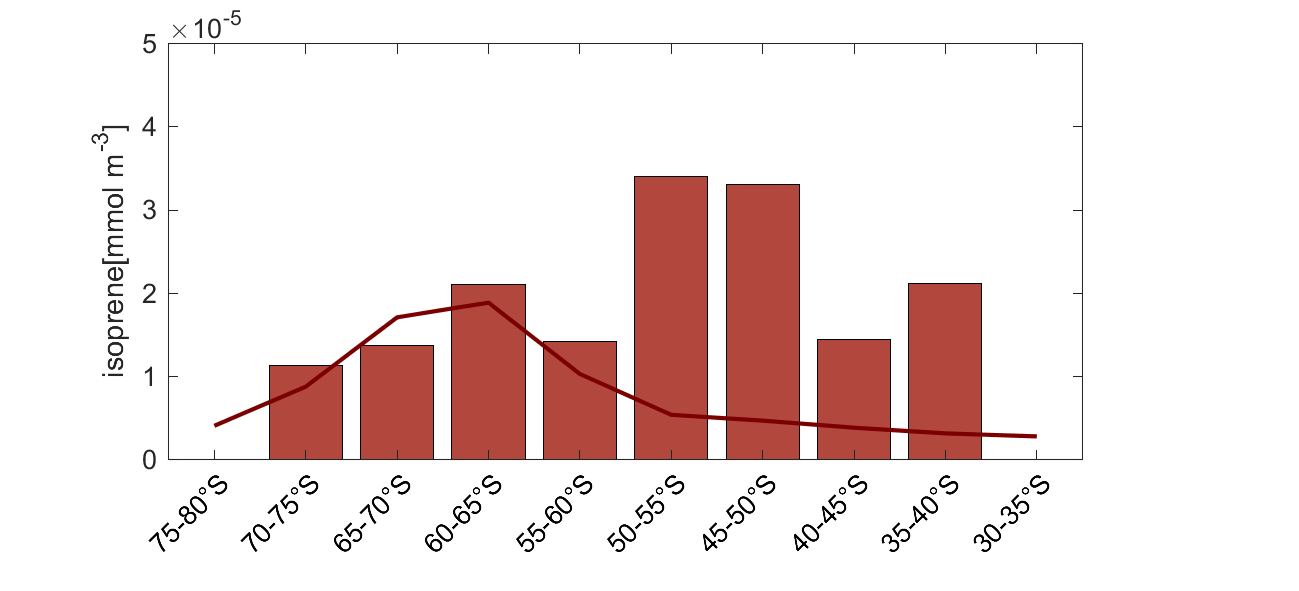
\includegraphics[width=.9\textwidth]{Plots/isoprene_zonal_avg_DJFM_top50m_SO_d05_017.png}
\caption{Model validation using in situ data of isoprene concentration from TransPEGASO, PEGASO and ACE Expedition. Bars: In situ data. Line: model data.}
\label{fig:validation.lat}
\end{figure}

\section{Discussion}

\subsubsection{The SO, PP and phytoplankton}

The southern ocean is the most productive ocean on earth (citation needed), reaching extremely high values of PP during summer. Since\\

The relevance of isoprene in an ocean which is likely to be the most important in terms of diatom diversity and abundance.\\

Carbon fixation by phytoplankton\\

However, the \textbf{lack of production rates of marine isoprene in the Southern Ocean} compiled in \citep{booge2016can} reflect that isoprene specific production by phytoplankton (and phytoplankton diversity and abundance patterns) must be improved in order to increase the quality of this modelling approach and others. There have been performed several analyses of isoprene production in the global ocean using data from many cruises \citep{hackenberg2017potential}. However, isoprene emissions in the Southern Ocean remain poorly constrained. All in all, we agree with \citep{ooki2015global} that there still is a paucity of relevant observations, making the prediction of global oceanic C5H8 emissions a present problem to be solved \citep{ooki2015global}.\\

Do we agree with other recent works? like \citep{hackenberg2017potential}, that have highlighted that the next approach to be used in order to quantify the global isoprene emission must be to perform a similar approach than this one, but using a \textbf{global model including the global distribution of PFTs}.\\

\subsubsection{The contribution of the SO}

In one hand, when comparing our results to the highest estimates of the global emission of isoprene \citep{luo2010numerical} our estimates for the southern ocean contributes XX\% to the total emission.  In the other hand, our estimates for the SO exceed by much the lowest estimates of isoprene from the global ocean \citep{Arnold2009,booge2016can,palmer2005quantifying,gantt2009new}.

Our results emission of isoprene from the SO suggest that there is still a huge discrepancy among the different works which needs to be solved. A global assessment based of PFT approaches must be performed in order to calculate more accurately the global emission 
of isoprene \citep{hackenberg2017potential}.

\begin{center}

\begin{table}[h!]

\centering

\caption{Global estimates of isoprene emissions for the Global Ocean in comparison with our preliminary results for the Southern Ocean [Rodriguez-Ros et al., 2018, in preparation]. A more updated verssion of global estimates of isoprene emission from the published bibliography can be found in \citep{bruggemann2018interfacial}.}
\bigskip

\label{tab:global}

\begin{tabular}[ht]{ c|c|c|c|c|c } 

 \textbf{Area} & \textbf{Reference} & \textbf{Range} & \textbf{Unit} & \textbf{Type} \\\hline

Southern Ocean & ISO.ROMS.BEC &  0.027  & 	Tg C yr -1 & Bottom-up  \\

Global Ocean & \citep{palmer2005quantifying}   & 0.1   &  Tg C yr -1 & Top-down \\

Global Ocean  & \citep{booge2016can}  & 0.21 & Tg C yr -1 &  Bottom-up\\

Global Ocean  & \citep{Arnold2009} & 0.31 - 1.9 & Tg C yr -1 & Bottom-up -- Top-down \\

Global Ocean  & \citep{luo2010numerical} & 0.32 - 11.6  & Tg C yr -1 &  Bottom-up -- Top-down \\
Global Ocean  & \citep{gantt2009new} & 1.9 & Tg C yr -1   & Bottom-up\\
Global Ocean  & \citep{bruggemann2018interfacial} & 0.70 - 1.52 & Tg C yr -1 & Bottom-up  \\
Global Ocean  & \citep{shaw2010production} & 0.085 - 11.6 & Tg C yr -1 & Bottom-up -- Top-down \\
\end{tabular}

\end{table}

\end{center}

\section{Conclusions}


%Text here ===>>>

%%

%  Numbered lines in equations:
%  To add line numbers to lines in equations,
%  \begin{linenomath*}
%  \begin{equation}
%  \end{equation}
%  \end{linenomath*}


%% Enter Figures and Tables near as possible to where they are first mentioned:
%
% DO NOT USE \psfrag or \subfigure commands.
%
% Figure captions go below the figure.
% Table titles go above tables;  other caption information
%  should be placed in last line of the table, using
% \multicolumn2l{$^a$ This is a table note.}
%
%----------------
% EXAMPLE FIGURE
%
% \begin{figure}[h]
% \centering
% when using pdflatex, use pdf file:
% 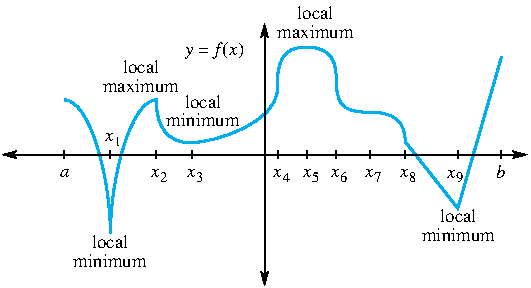
\includegraphics[width=20pc]{figsamp.pdf}
%
% when using dvips, use .eps file:
% 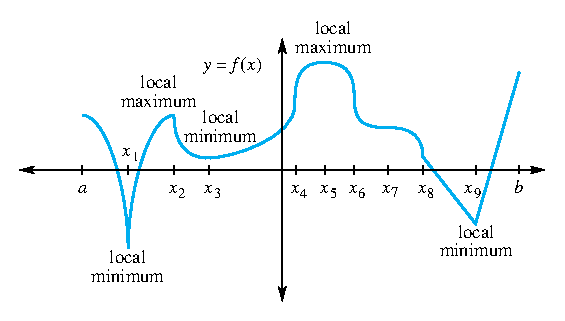
\includegraphics[width=20pc]{figsamp.eps}
%
% \caption{Short caption}
% \label{figone}
%  \end{figure}
%
% ---------------
% EXAMPLE TABLE
%
% \begin{table}
% \caption{Time of the Transition Between Phase 1 and Phase 2$^{a}$}
% \centering
% \begin{tabular}{l c}
% \hline
%  Run  & Time (min)  \\
% \hline
%   $l1$  & 260   \\
%   $l2$  & 300   \\
%   $l3$  & 340   \\
%   $h1$  & 270   \\
%   $h2$  & 250   \\
%   $h3$  & 380   \\
%   $r1$  & 370   \\
%   $r2$  & 390   \\
% \hline
% \multicolumn{2}{l}{$^{a}$Footnote text here.}
% \end{tabular}
% \end{table}

%% SIDEWAYS FIGURE and TABLE 
% AGU prefers the use of {sidewaystable} over {landscapetable} as it causes fewer problems.
%
% \begin{sidewaysfigure}
% 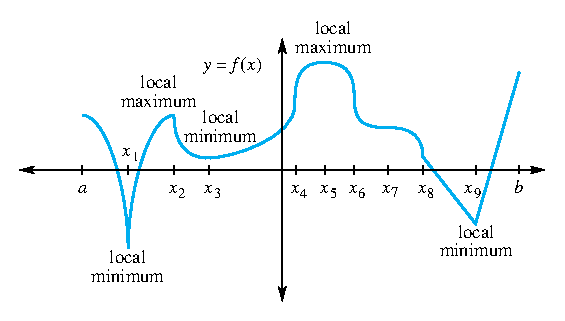
\includegraphics[width=20pc]{figsamp}
% \caption{caption here}
% \label{newfig}
% \end{sidewaysfigure}
% 
%  \begin{sidewaystable}
%  \caption{Caption here}
% \label{tab:signif_gap_clos}
%  \begin{tabular}{ccc}
% one&two&three\\
% four&five&six
%  \end{tabular}
%  \end{sidewaystable}

%% If using numbered lines, please surround equations with \begin{linenomath*}...\end{linenomath*}
%\begin{linenomath*}
%\begin{equation}
%y|{f} \sim g(m, \sigma),
%\end{equation}
%\end{linenomath*}

%%% End of body of article

%%%%%%%%%%%%%%%%%%%%%%%%%%%%%%%%
%% Optional Appendix goes here
%
% The \appendix command resets counters and redefines section heads
%
% After typing \appendix
%
%\section{Here Is Appendix Title}
% will show
% A: Here Is Appendix Title
%
%\appendix
%\section{Here is a sample appendix}

%%%%%%%%%%%%%%%%%%%%%%%%%%%%%%%%%%%%%%%%%%%%%%%%%%%%%%%%%%%%%%%%
%
% Optional Glossary, Notation or Acronym section goes here:
%
%%%%%%%%%%%%%%  
% Glossary is only allowed in Reviews of Geophysics
%  \begin{glossary}
%  \term{Term}
%   Term Definition here
%  \term{Term}
%   Term Definition here
%  \term{Term}
%   Term Definition here
%  \end{glossary}

%
%%%%%%%%%%%%%%
% Acronyms
%   \begin{acronyms}
%   \acro{Acronym}
%   Definition here
%   \acro{EMOS}
%   Ensemble model output statistics 
%   \acro{ECMWF}
%   Centre for Medium-Range Weather Forecasts
%   \end{acronyms}

%
%%%%%%%%%%%%%%
% Notation 
%   \begin{notation}
%   \notation{$a+b$} Notation Definition here
%   \notation{$e=mc^2$} 
%   Equation in German-born physicist Albert Einstein's theory of special
%  relativity that showed that the increased relativistic mass ($m$) of a
%  body comes from the energy of motion of the body—that is, its kinetic
%  energy ($E$)—divided by the speed of light squared ($c^2$).
%   \end{notation}




%%%%%%%%%%%%%%%%%%%%%%%%%%%%%%%%%%%%%%%%%%%%%%%%%%%%%%%%%%%%%%%%
%
%  ACKNOWLEDGMENTS
%
% The acknowledgments must list:
%
% •	All funding sources related to this work from all authors
%
% •	Any real or perceived financial conflicts of interests for any
%	author
%
% •	Other affiliations for any author that may be perceived as
% 	having a conflict of interest with respect to the results of this
% 	paper.
%
% •	A statement that indicates to the reader where the data
% 	supporting the conclusions can be obtained (for example, in the
% 	references, tables, supporting information, and other databases).
%
% It is also the appropriate place to thank colleagues and other contributors. 
% AGU does not normally allow dedications.


\acknowledgments
HERE

%% ------------------------------------------------------------------------ %%
%% Citations

% Please use ONLY \citet and \citep for reference citations.
% DO NOT use other cite commands (e.g., \cite, \citeyear, \nocite, \citealp, etc.).


%% Example \citet and \citep:
%  ...as shown by \citet{Boug10}, \citet{Buiz07}, \citet{Fra10},
%  \citet{Ghel00}, and \citet{Leit74}. 

%  ...as shown by \citep{Boug10}, \citep{Buiz07}, \citep{Fra10},
%  \citep{Ghel00, Leit74}. 

%  ...has been shown \citep [e.g.,][]{Boug10,Buiz07,Fra10}.



%%  REFERENCE LIST AND TEXT CITATIONS
\bibliography{mybib.bib}
%
% Either type in your references using
%
% \begin{thebibliography}{}
% \bibitem[{\textit{Kobayashi et~al.}}(2003)]{R2013} Kobayashi, T.,
% Tran, A.~H., Nishijo, H., Ono, T., and Matsumoto, G.  (2003).
% Contribution of hippocampal place cell activity to learning and
% formation of goal-directed navigation in rats. \textit{Neuroscience}
% 117, 1025--1035.
%
% \bibitem{}
% Text
% \end{thebibliography}
%
%%%%%%%%%%%%%%%%%%%%%%%%%%%%%%%%%%%%%%%%%%%%%%%
% Or, to use BibTeX:
%
% Follow these steps
%
% 1. Type in \bibliography{<name of your .bib file>} 
%    Run LaTeX on your LaTeX file.
%
% 2. Run BiBTeX on your LaTeX file.
%
% 3. Open the new .bbl file containing the reference list and
%   copy all the contents into your LaTeX file here.
%
% 4. Run LaTeX on your new file which will produce the citations.
%
% AGU does not want a .bib or a .bbl file. Please copy in the contents of your .bbl file here.


%% After you run BibTeX, Copy in the contents of the .bbl file here:


%%%%%%%%%%%%%%%%%%%%%%%%%%%%%%%%%%%%%%%%%%%%%%%%%%%%%%%%%%%%%%%%%%%%%
% Track Changes:
% To add words, \added{<word added>}
% To delete words, \deleted{<word deleted>}
% To replace words, \replaced{<word to be replaced>}{<replacement word>}
% To explain why change was made: \explain{<explanation>} This will put
% a comment into the right margin.

%%%%%%%%%%%%%%%%%%%%%%%%%%%%%%%%%%%%%%%%%%%%%%%%%%%%%%%%%%%%%%%%%%%%%
% At the end of the document, use \listofchanges, which will list the
% changes and the page and line number where the change was made.

% When final version, \listofchanges will not produce anything,
% \added{<word or words>} word will be printed, \deleted{<word or words} will take away the word,
% \replaced{<delete this word>}{<replace with this word>} will print only the replacement word.
%  In the final version, \explain will not print anything.
%%%%%%%%%%%%%%%%%%%%%%%%%%%%%%%%%%%%%%%%%%%%%%%%%%%%%%%%%%%%%%%%%%%%%

%%%
\listofchanges
%%%

\end{document}

%%%%%%%%%%%%%%%%%%%%%%%%%%%%%%%%%%%%%
%% Supporting Information
%% (Optional) See AGUSuppInfoSamp.tex/pdf for requirements 
%% for Supporting Information.
%%%%%%%%%%%%%%%%%%%%%%%%%%%%%%%%%%%%%



%%%%%%%%%%%%%%%%%%%%%%%%%%%%%%%%%%%%%%%%%%%%%%%%%%%%%%%%%%%%%%%

More Information and Advice:

%% ------------------------------------------------------------------------ %%
%
%  SECTION HEADS
%
%% ------------------------------------------------------------------------ %%

% Capitalize the first letter of each word (except for
% prepositions, conjunctions, and articles that are
% three or fewer letters).

% AGU follows standard outline style; therefore, there cannot be a section 1 without
% a section 2, or a section 2.3.1 without a section 2.3.2.
% Please make sure your section numbers are balanced.
% ---------------
% Level 1 head
%
% Use the \section{} command to identify level 1 heads;
% type the appropriate head wording between the curly
% brackets, as shown below.
%
%An example:
%\section{Level 1 Head: Introduction}
%
% ---------------
% Level 2 head
%
% Use the \subsection{} command to identify level 2 heads.
%An example:
%\subsection{Level 2 Head}
%
% ---------------
% Level 3 head
%
% Use the \subsubsection{} command to identify level 3 heads
%An example:
%\subsubsection{Level 3 Head}
%
%---------------
% Level 4 head
%
% Use the \subsubsubsection{} command to identify level 3 heads
% An example:
%\subsubsubsection{Level 4 Head} An example.
%
%% ------------------------------------------------------------------------ %%
%
%  IN-TEXT LISTS
%
%% ------------------------------------------------------------------------ %%
%
% Do not use bulleted lists; enumerated lists are okay.
% \begin{enumerate}
% \item
% \item
% \item
% \end{enumerate}
%
%% ------------------------------------------------------------------------ %%
%
%  EQUATIONS
%
%% ------------------------------------------------------------------------ %%

% Single-line equations are centered.
% Equation arrays will appear left-aligned.

Math coded inside display math mode \[ ...\]
 will not be numbered, e.g.,:
 \[ x^2=y^2 + z^2\]

 Math coded inside \begin{equation} and \end{equation} will
 be automatically numbered, e.g.,:
 \begin{equation}
 x^2=y^2 + z^2
 \end{equation}


% To create multiline equations, use the
% \begin{eqnarray} and \end{eqnarray} environment
% as demonstrated below.
\begin{eqnarray}
  x_{1} & = & (x - x_{0}) \cos \Theta \nonumber \\
        && + (y - y_{0}) \sin \Theta  \nonumber \\
  y_{1} & = & -(x - x_{0}) \sin \Theta \nonumber \\
        && + (y - y_{0}) \cos \Theta.
\end{eqnarray}

%If you don't want an equation number, use the star form:
%\begin{eqnarray*}...\end{eqnarray*}

% Break each line at a sign of operation
% (+, -, etc.) if possible, with the sign of operation
% on the new line.

% Indent second and subsequent lines to align with
% the first character following the equal sign on the
% first line.

% Use an \hspace{} command to insert horizontal space
% into your equation if necessary. Place an appropriate
% unit of measure between the curly braces, e.g.
% \hspace{1in}; you may have to experiment to achieve
% the correct amount of space.


%% ------------------------------------------------------------------------ %%
%
%  EQUATION NUMBERING: COUNTER
%
%% ------------------------------------------------------------------------ %%

% You may change equation numbering by resetting
% the equation counter or by explicitly numbering
% an equation.

% To explicitly number an equation, type \eqnum{}
% (with the desired number between the brackets)
% after the \begin{equation} or \begin{eqnarray}
% command.  The \eqnum{} command will affect only
% the equation it appears with; LaTeX will number
% any equations appearing later in the manuscript
% according to the equation counter.
%

% If you have a multiline equation that needs only
% one equation number, use a \nonumber command in
% front of the double backslashes (\\) as shown in
% the multiline equation above.

% If you are using line numbers, remember to surround
% equations with \begin{linenomath*}...\end{linenomath*}

%  To add line numbers to lines in equations:
%  \begin{linenomath*}
%  \begin{equation}
%  \end{equation}
%  \end{linenomath*}



